\documentclass{ctexart}
\usepackage{amsmath}
\usepackage{float}
\usepackage{amssymb}
\usepackage{graphicx}
\usepackage{gbt7714}
\usepackage{pifont}
\usepackage{wrapfig}
\usepackage{multirow}
\ctexset{
    % 修改 section。
    section={   
        name={,、},
        number={\chinese{section}}
    }
}

\title{分光计测定棱镜的折射率}
\author{陆知辰-10225301478}
\date{\today}
\graphicspath{{figure/}}

\begin{document}

\begin{titlepage}
  \centering
  % 插入图片
  
\includegraphics[width=0.5\textwidth]{ecnu.png}
  
  % 空行用于调整标题位置
  \vspace*{\baselineskip}
  
  % 标题
  \Huge\textbf{物\quad 理\quad 实\quad 验 \quad (二)}
  % 空行用于调整标题和其他信息之间的间距
  \vspace*{0.3\baselineskip}
  
  % 具体实验名称
  \huge 分光计测定棱镜的折射率
  
  % 空行用于调整时间和其他信息之间的间距
  \vspace*{2\baselineskip}
  
  % 时间
  \large 时间:\today
  
  % 空行用于调整时间和其他信息之间的间距
  \vspace*{\baselineskip}
  
  % 创作人
  \large 创作人:陆知辰
  
  % 空行用于调整创作人和学号之间的间距
  \vspace*{\baselineskip}
  
  % 学号
  \large 学号:10225301478
  
\end{titlepage}
\newpage
\tableofcontents
\newpage
\section{实验摘要}
  \subsection{实验概要}
  分光计是比较精密的仪器,构造精细、调节技术要求高,能精确测定光线偏转角,
  可以用于测量材料的折射率、光源的光谱,它在光的反射、折射、干涉、偏振实验以及对某些材料的研究中具有重要应用。
  本实验要求实验者正确调整和使用分光计,利用分光计观察棱镜的色散光谱,测量棱镜对某些波长的光的折射率,并进一步理解折射率的大小与光波波长有关这一概念.
  \subsection{实验目的}
  1.\quad 在分光计的调节中,为什么要先调节望远镜,在调节平台,最后调节平行光管。

  2.\quad 如果将分光计的结构与夫琅禾费衍射的光路进行对比,两者有何相似的地方?
  
  3.\quad 分光计处于待测量状态的标志有哪些?

\section{实验原理}
  \subsection{最小偏向角}
  \begin{figure}[H]
    \centering
    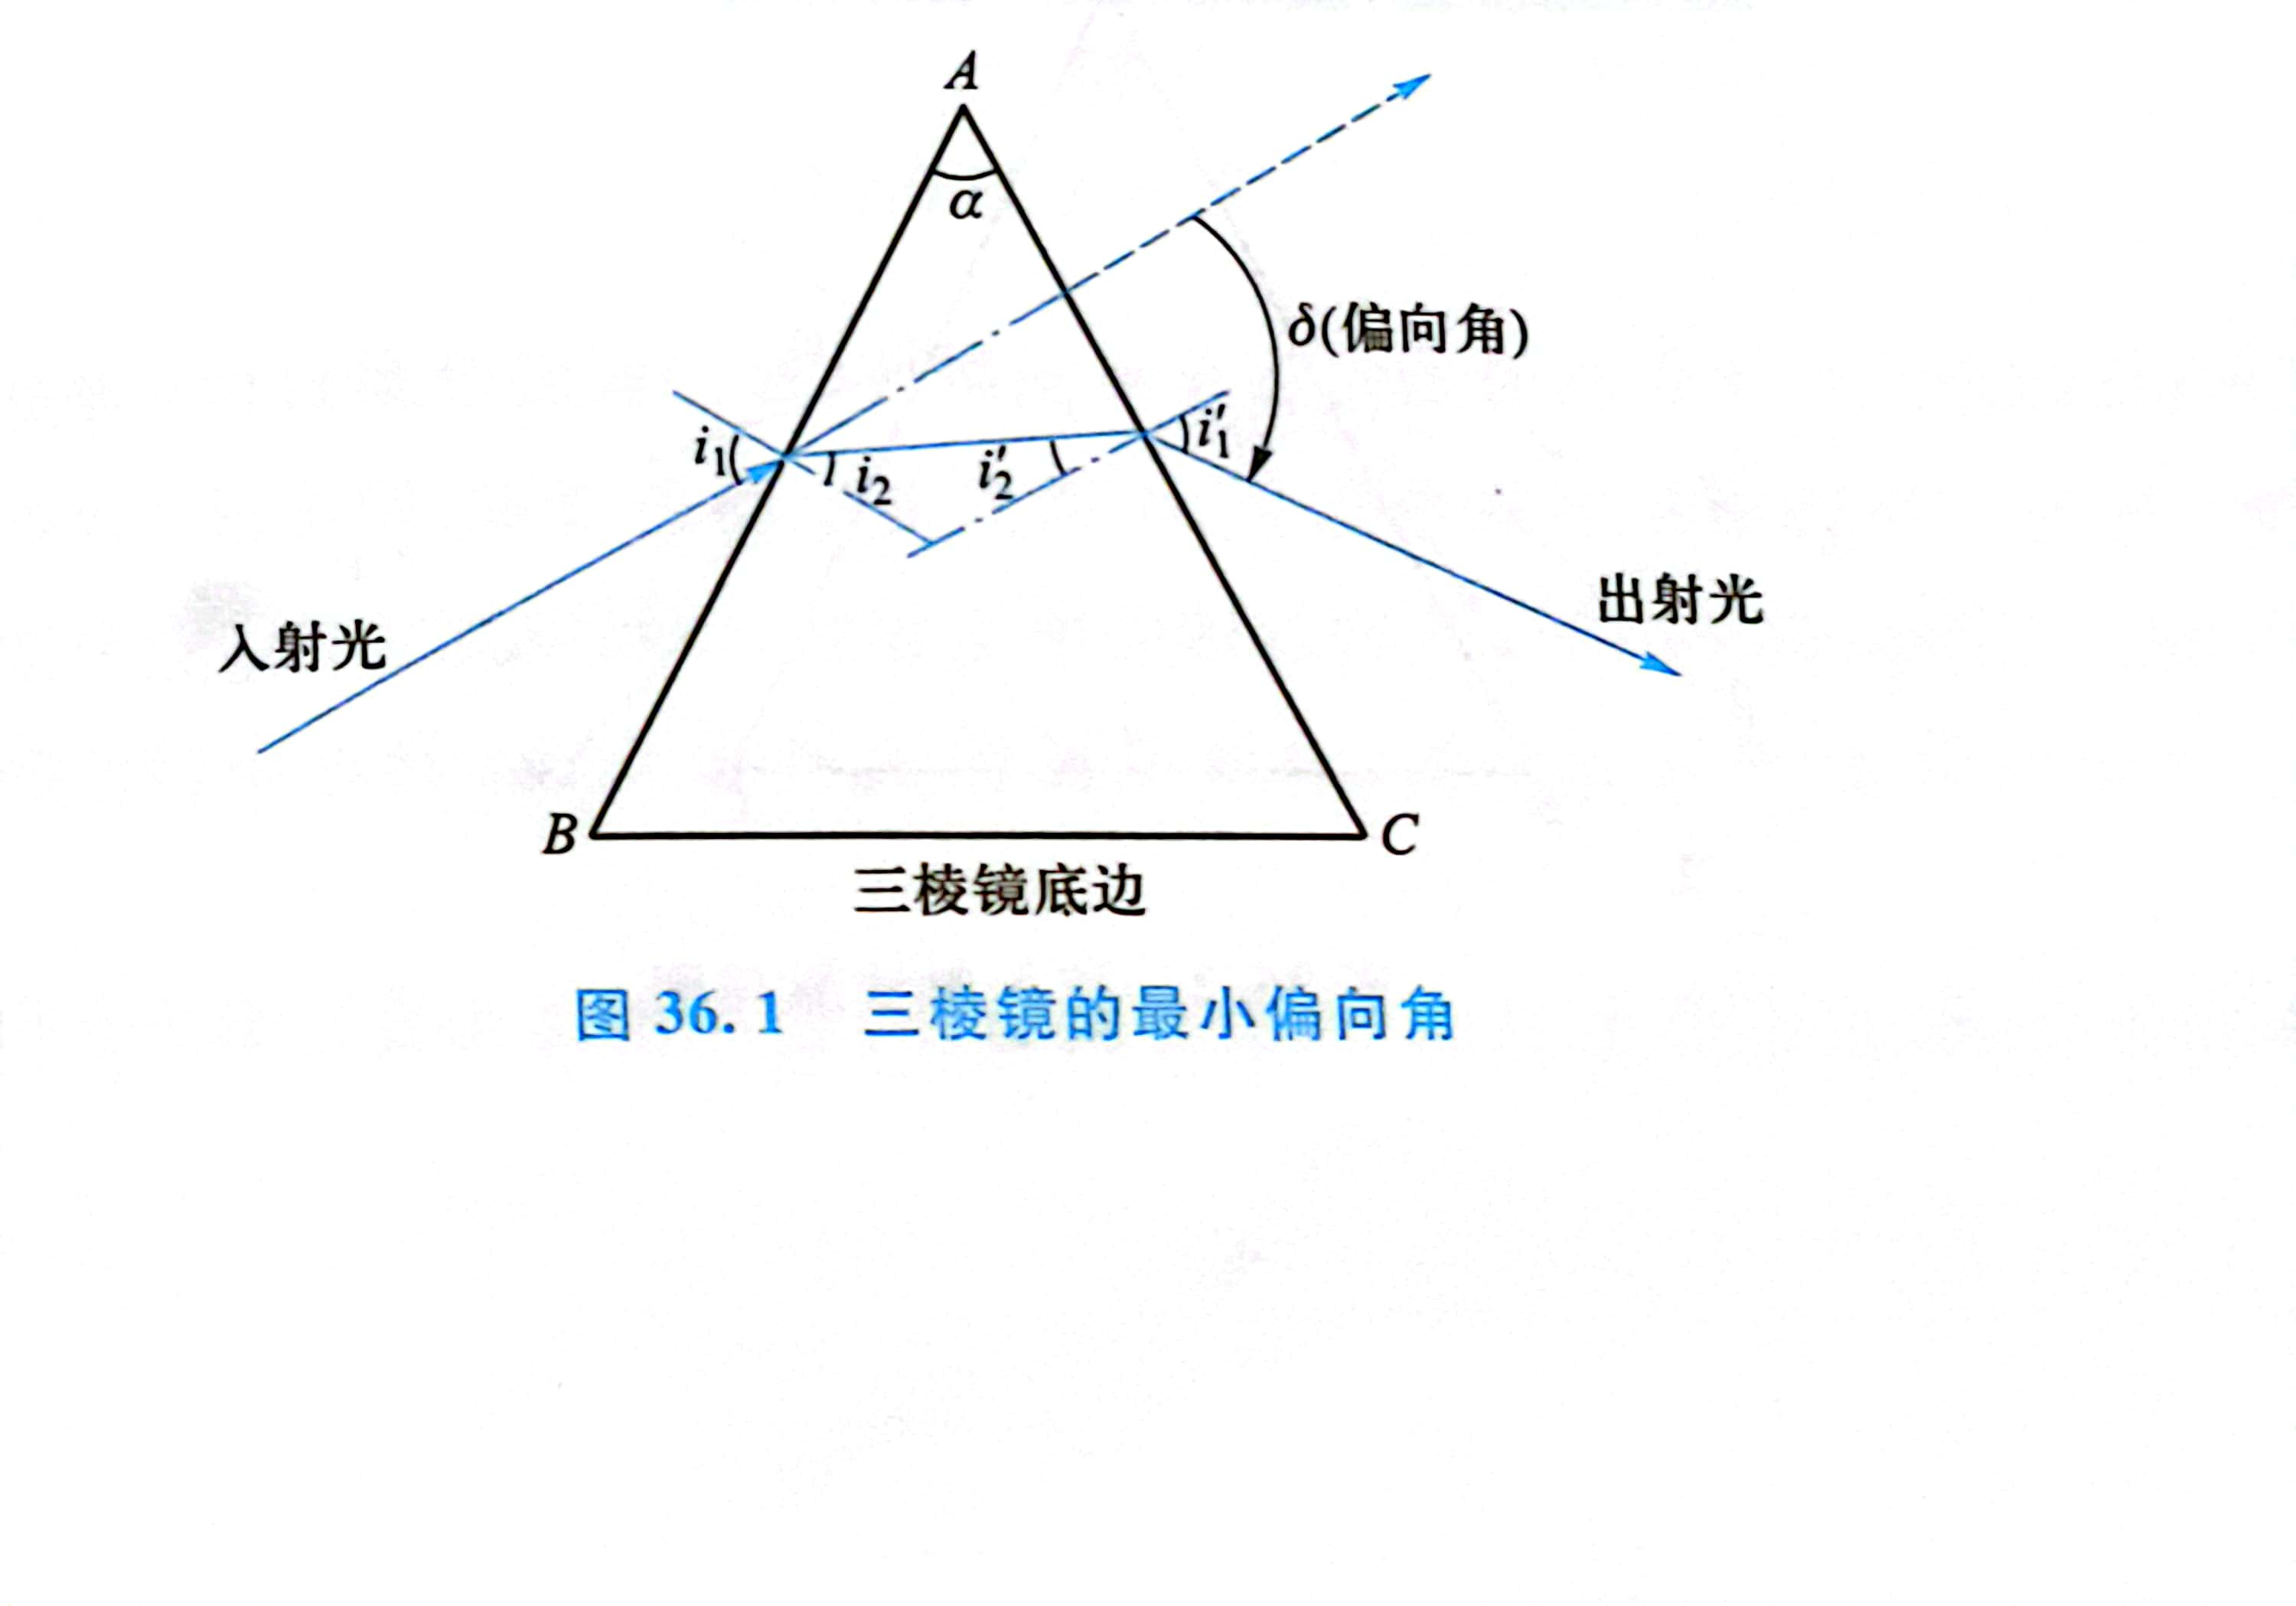
\includegraphics[height=0.6\textwidth,width=1\textwidth]{zuixiaopianxiangjiao.jpg}
    \caption{三棱镜的最小偏向角}\label{zuixiaopianxiangjiao}
  \end{figure}
  如图\ref{zuixiaopianxiangjiao}所示,当一束波长为入的光从三棱镜的一侧AB面以入射角记人射时,
  由于折射角$i_{2}$小于人射角$i_{2}$,所以该光束进入三棱镜后会向底边方向偏转.
  当该光束进一步人射到另一侧面AC并以入射角${i}_{2}^{'}$向空气出射时,由于此时折射角${i}_{1}^{'}$和
  大于人射角$i_{2}^{'}$,所以会使得光线进一步向底边方向偏转,入射光和出射光之间的夹角称为偏向角,在图\ref{zuixiaopianxiangjiao}中用$\delta$表示。
  根据光线的可逆性原理,当入射光线和出射光线相对于三棱镜对称时,偏向角$\delta$存在最小值,称之为最小偏向角,用$\delta_{min}$表示,在此条件下,
  $i_{1}=i_{1}^{'}$,$i_{2}=i_{2}^{'}$.若三棱镜的顶角为$\alpha$,则有$i_{2}=\frac{\alpha}{2}$,$i_{1}=\frac{\alpha + \delta_{min}}{2}$。
  
  由折射定理可知,三棱镜对波长为$\lambda$的光的折射率$n$由下式给出:
  \begin{equation}\label{zheshelv1}
    n=\frac{\sin\frac{\alpha+\delta_{min}}{2}}{\sin\frac{\alpha}{2}}
  \end{equation}
  在实验中只要测出三棱镜的顶角$\alpha$和相应光线的最小偏向角$\delta_{min}$,即可由式\ref{zheshelv1}求出棱镜对该波长光的折射率。

  \subsection{掠入射法}
  \begin{figure}[H]
    \centering
    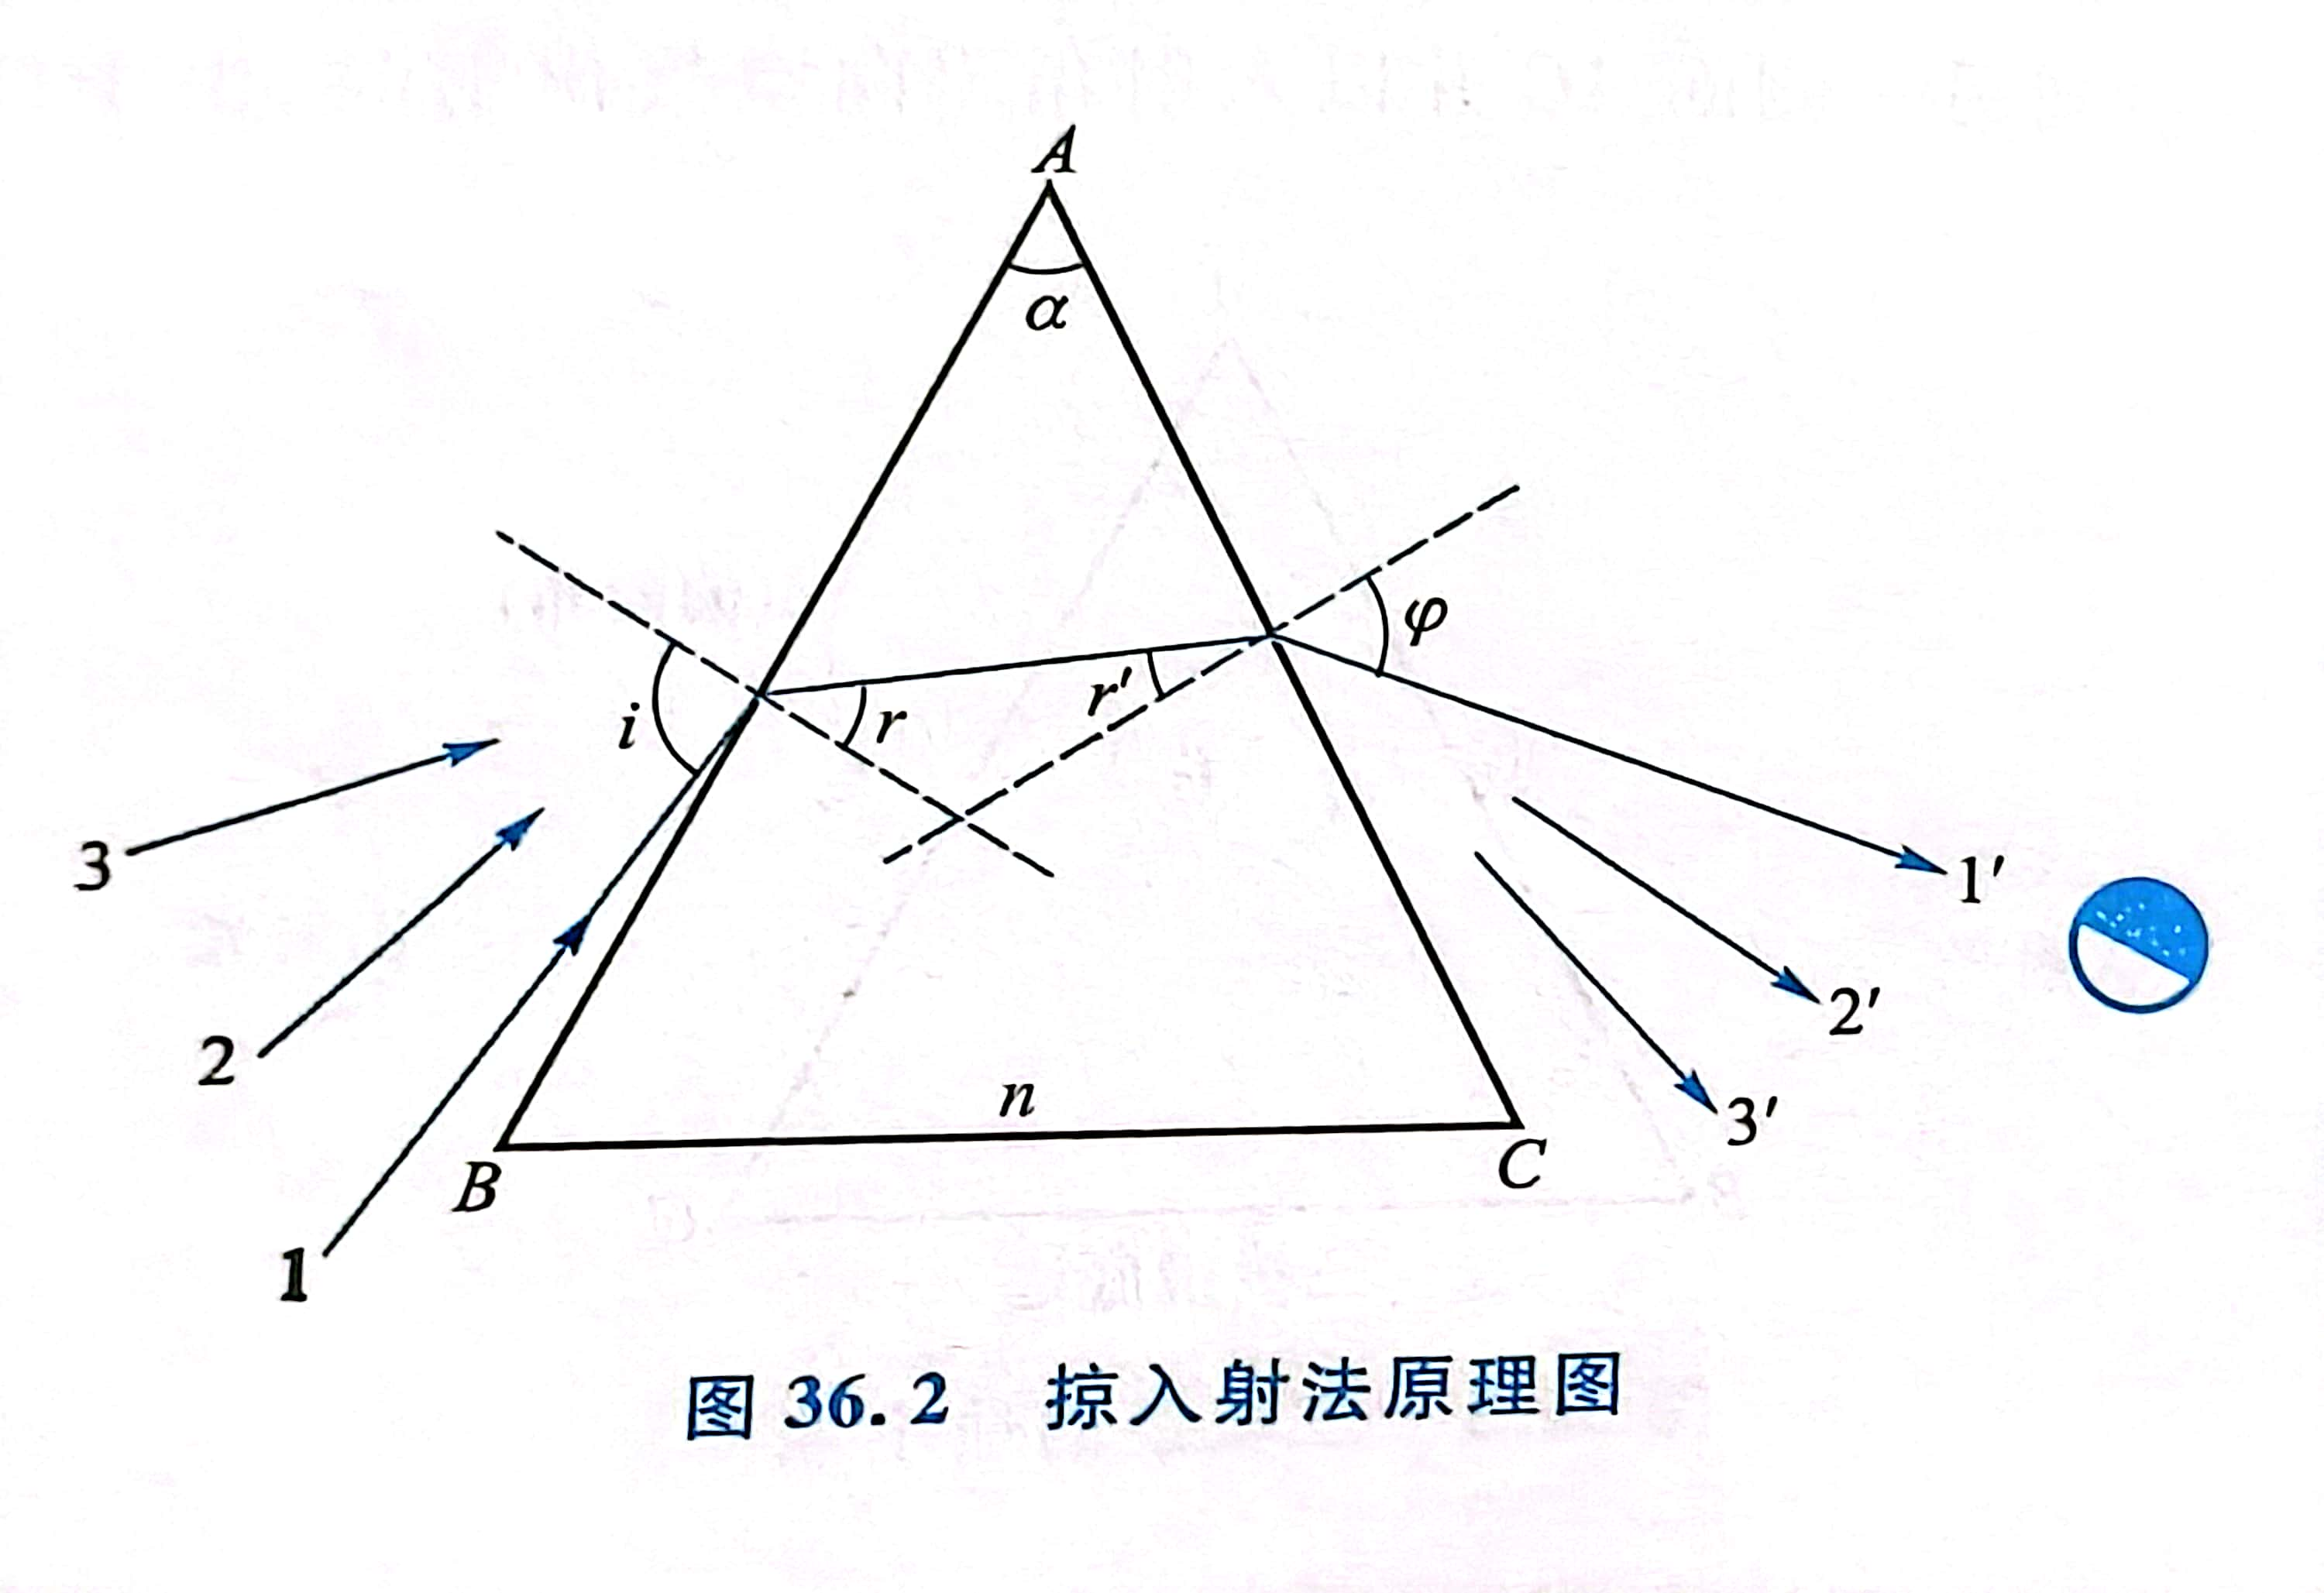
\includegraphics[height=0.6\textwidth,width=1\textwidth]{luerushefa.jpg}
    \caption{掠入射法示意图}\label{luerushefa}
  \end{figure}
  当扩展光源的光线,如图\ref{luerushefa}中的光线1-3,从三棱镜的一侧光学面AB入射三棱镜时,根据前面的分析,入射角i<90°
  的光线会经过一系列的折射后从三棱镜的另一侧AG面出射.对于入射角i=90°的光线,折射角满足关系式$n\sin r =1$.在AC面,
  折射角$\varphi$与入射角r'满足$n\sin r^{'}=\sin \varphi$.又因为在图\ref{luerushefa}中有$r+r^{'}=\alpha$,
  因此可求解得到i=90°的光线出射角$\alpha$满足的表达式为$\sin^{2}\alpha=n^{2}\sin^{2}\alpha-(\sin\varphi+\cos\alpha)^{2}$,
  因而,如果在实验中测量得到$\varphi$的值,即可得到三楼镜的折射率为
  \begin{equation}\label{zheshelv2}
    n=\frac{1}{\sin\alpha}\sqrt{\sin^{2}\alpha+(\sin\varphi+\cos\alpha)^{2}}
  \end{equation}
  由于不会有入射角大于90°的光线,因而光线在AC面出射后不会有折射角小于$\varphi$的光线,故从 AG 面一侧观察出射光时,会发现视场是半明半暗的,视场中间有明显的明暗分界线.

\section{实验装置器材介绍}
分光计一台,待测三校镜一块,反射平面镜两块,低压汞灯一台,低压钠灯一合,毛玻璃一块。

图\ref{yiqijiegou}为分光计的结构图和实物图,它主要由位于结构图左边的望远镜部分、
位于结构图中间的载物平台系统和位于结构图右边的平行光管部分构成。
\begin{figure}[H]
  \centering
  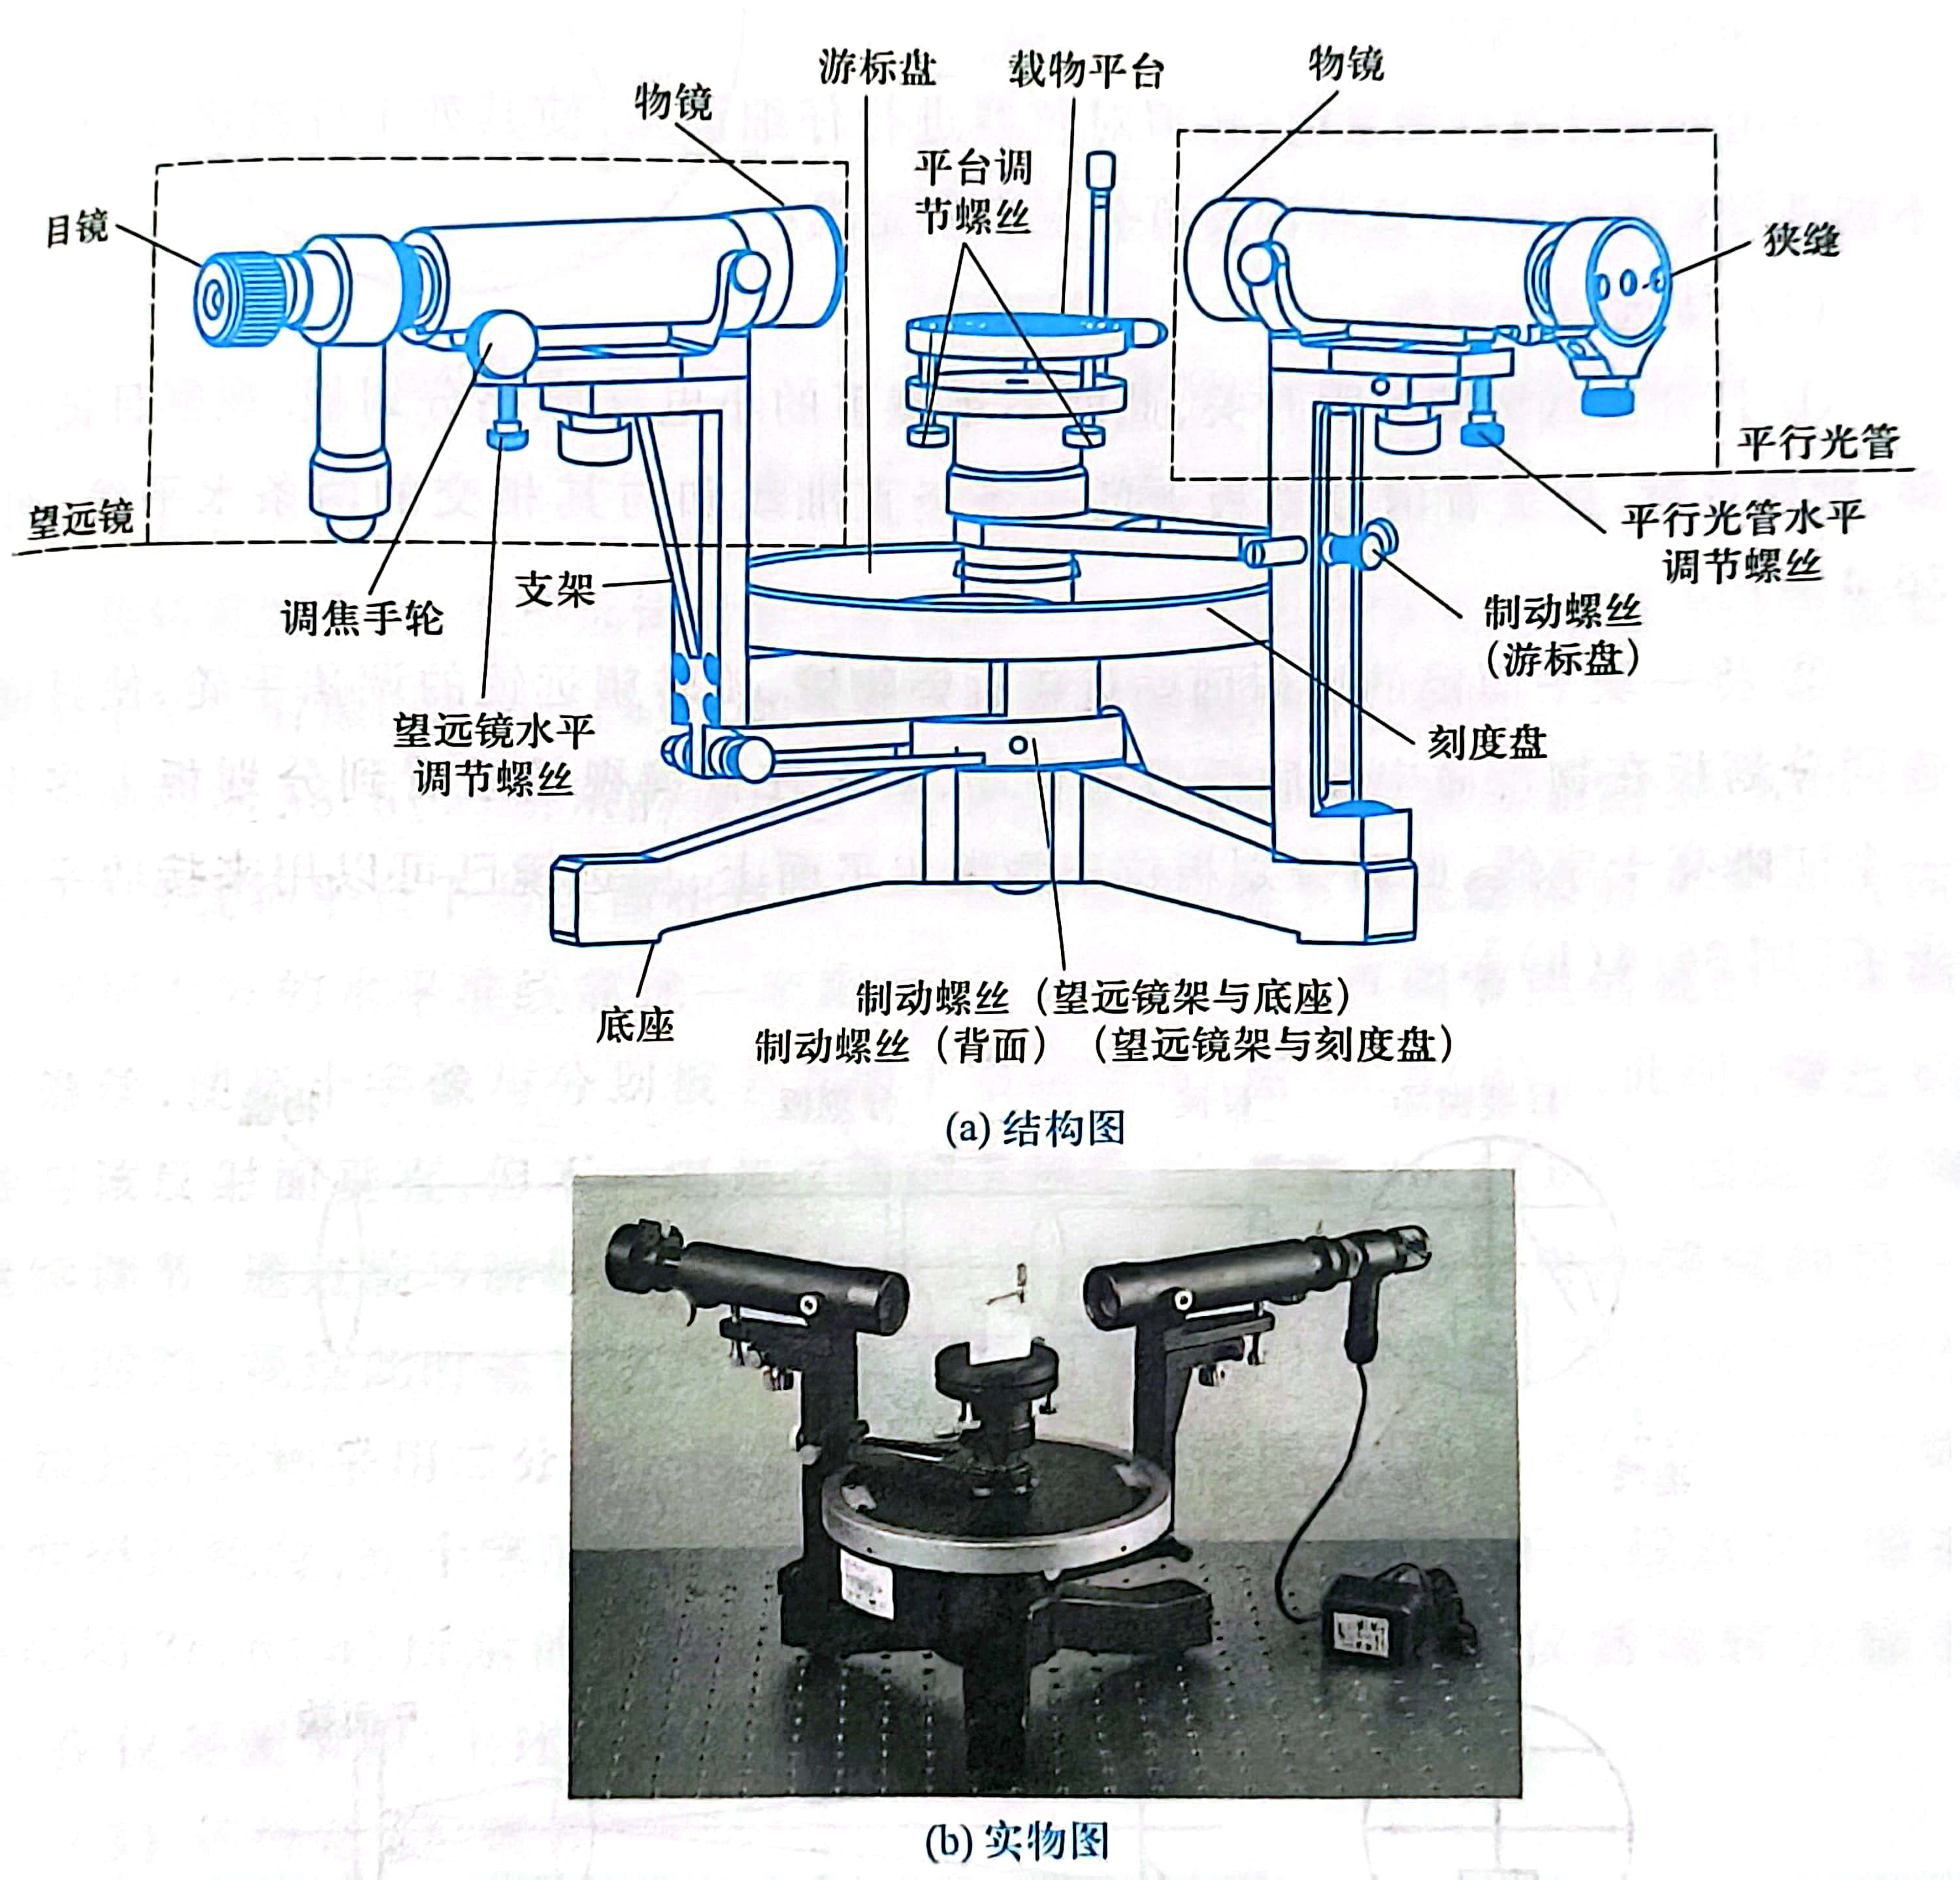
\includegraphics[height=1.2\textwidth,width=1\textwidth]{yiqijiegou.jpg}
  \caption{分光计仪器及其结构}\label{yiqijiegou}
\end{figure}

望远镜部分由目镜和物镜组成,目镜的调节通过旋转目镜实现,物镜的调节则通过旋转调焦手轮实现。
望远镜固定在支架上,可以绕载物平台的中心旋转,载物平台的前后分别有两个制动螺丝,旋紧正面的制动螺丝,
可以使望远镜和支架不能再绕载物平台的中心转动;旋紧背面的制动螺丝,则会使刻度盘和支架固定在一起,
载物平台系统主要由载物平台、平台调节螺丝、游标盘等构成,通过平台调节螺丝可以调节平台的水平状态,
利用游标盘可以读出待测位置的角坐标,当旋紧位
于平行光管下的制动螺丝时,载物平台和游标盘将不能绕转轴转动.
平行光管部分主要由物镜、狭缝和支架等组成,狭缝宽度可调,平行光管固定在支架上并和底座相连.

\section{实验内容及实验步骤}
  \subsection{分光计的调整}
  在用分光计进行测量前,必须对仪器进行仔细调整,使其处于待测状态,否则不能进行有效的测量,这种调整可分三步来完成。
    \subsubsection{望远镜的调整}
    示意图可以参考图\ref{wangyuanjingjiegou}。
    \begin{figure}[H]
      \centering
      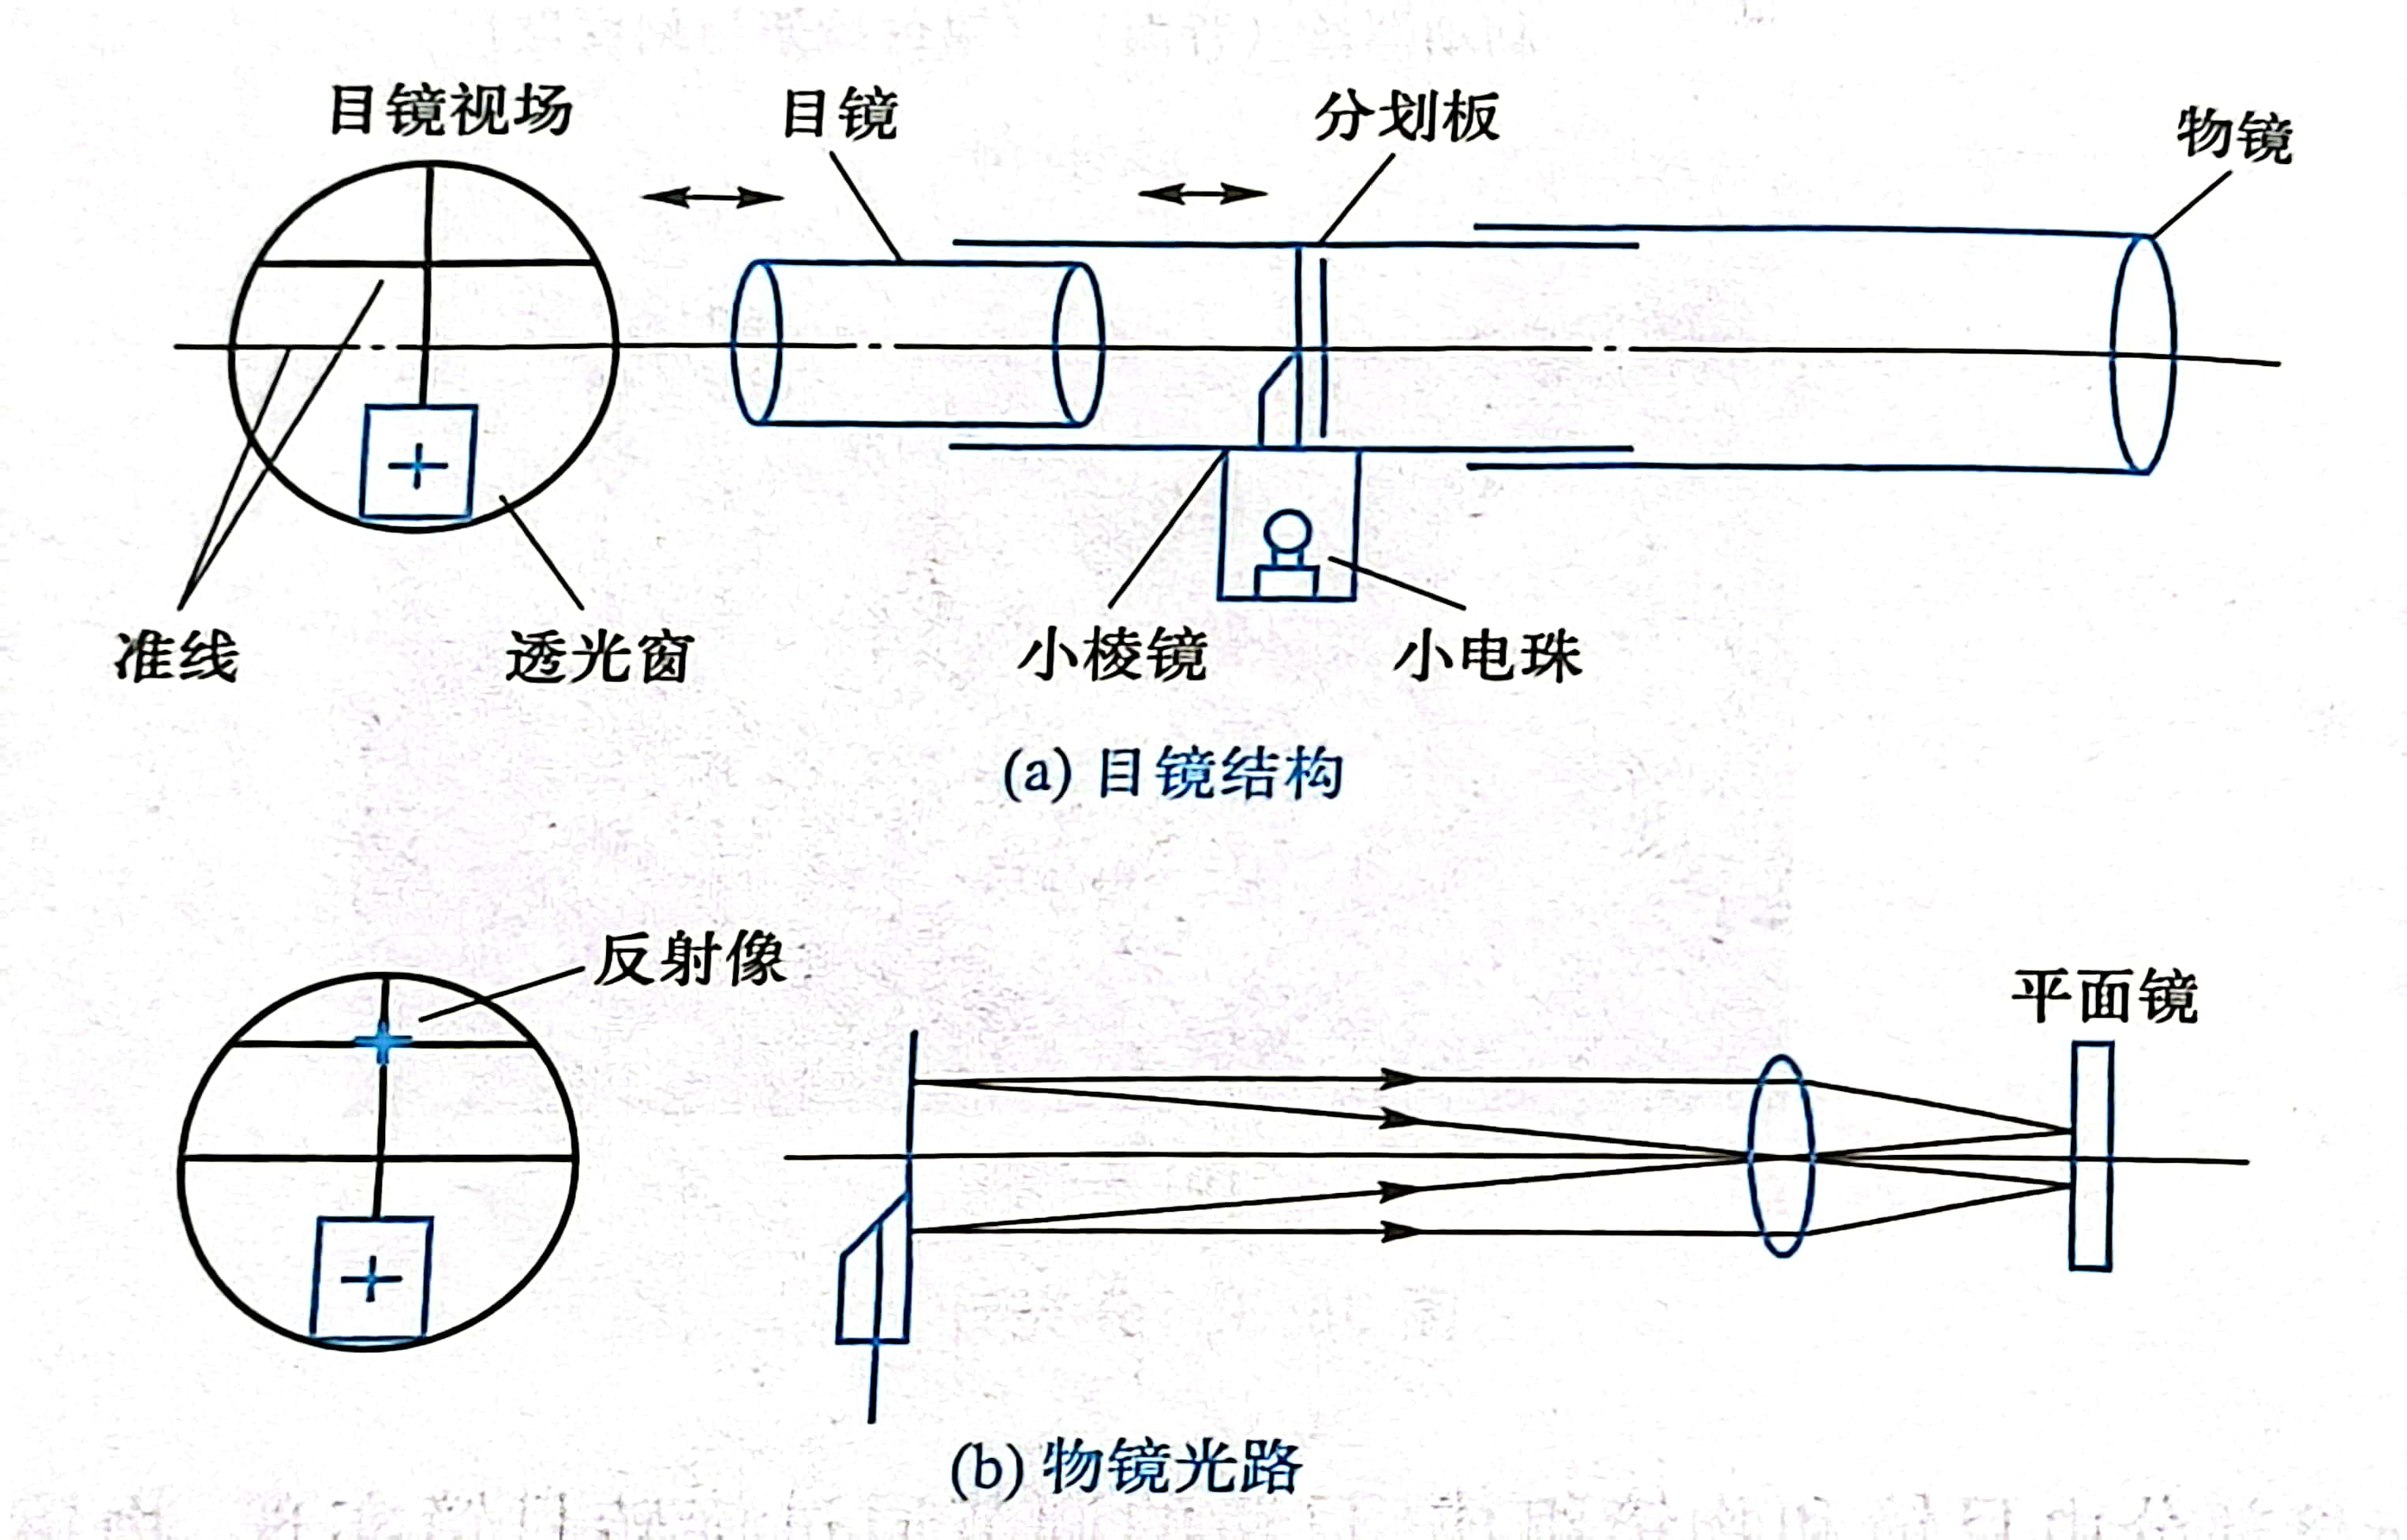
\includegraphics[height=0.4\textwidth,width=1\textwidth]{wangyuanjingjiegou.jpg}
      \caption{望远镜结构示意图}\label{wangyuanjingjiegou}
    \end{figure}

    1、 打开望远镜的照明开关,此时望远镜下的小电珠照亮分划板.观察目镜内部,旋转目镜,直至看清分划板上的一条竖直准线和与其相交的两条水平线。

    2、 将一块平面镜的反射面贴近望远镜物镜,旋转望远镜的调焦手轮,使目镜连同分划板在物镜筒中前后缓慢地移动,
    直至在目镜视场里看到分划板上多出一个清晰亮十字线,此时分划板位于物镜焦平面上,望远镜已可以用来接收平行光了。

    \subsubsection{调节望远镜的光轴与仪器旋转主轴垂直}
    示意图可以参考图\ref{tiaojiewangyuanjing}。
    \begin{figure}[H]
      \centering
      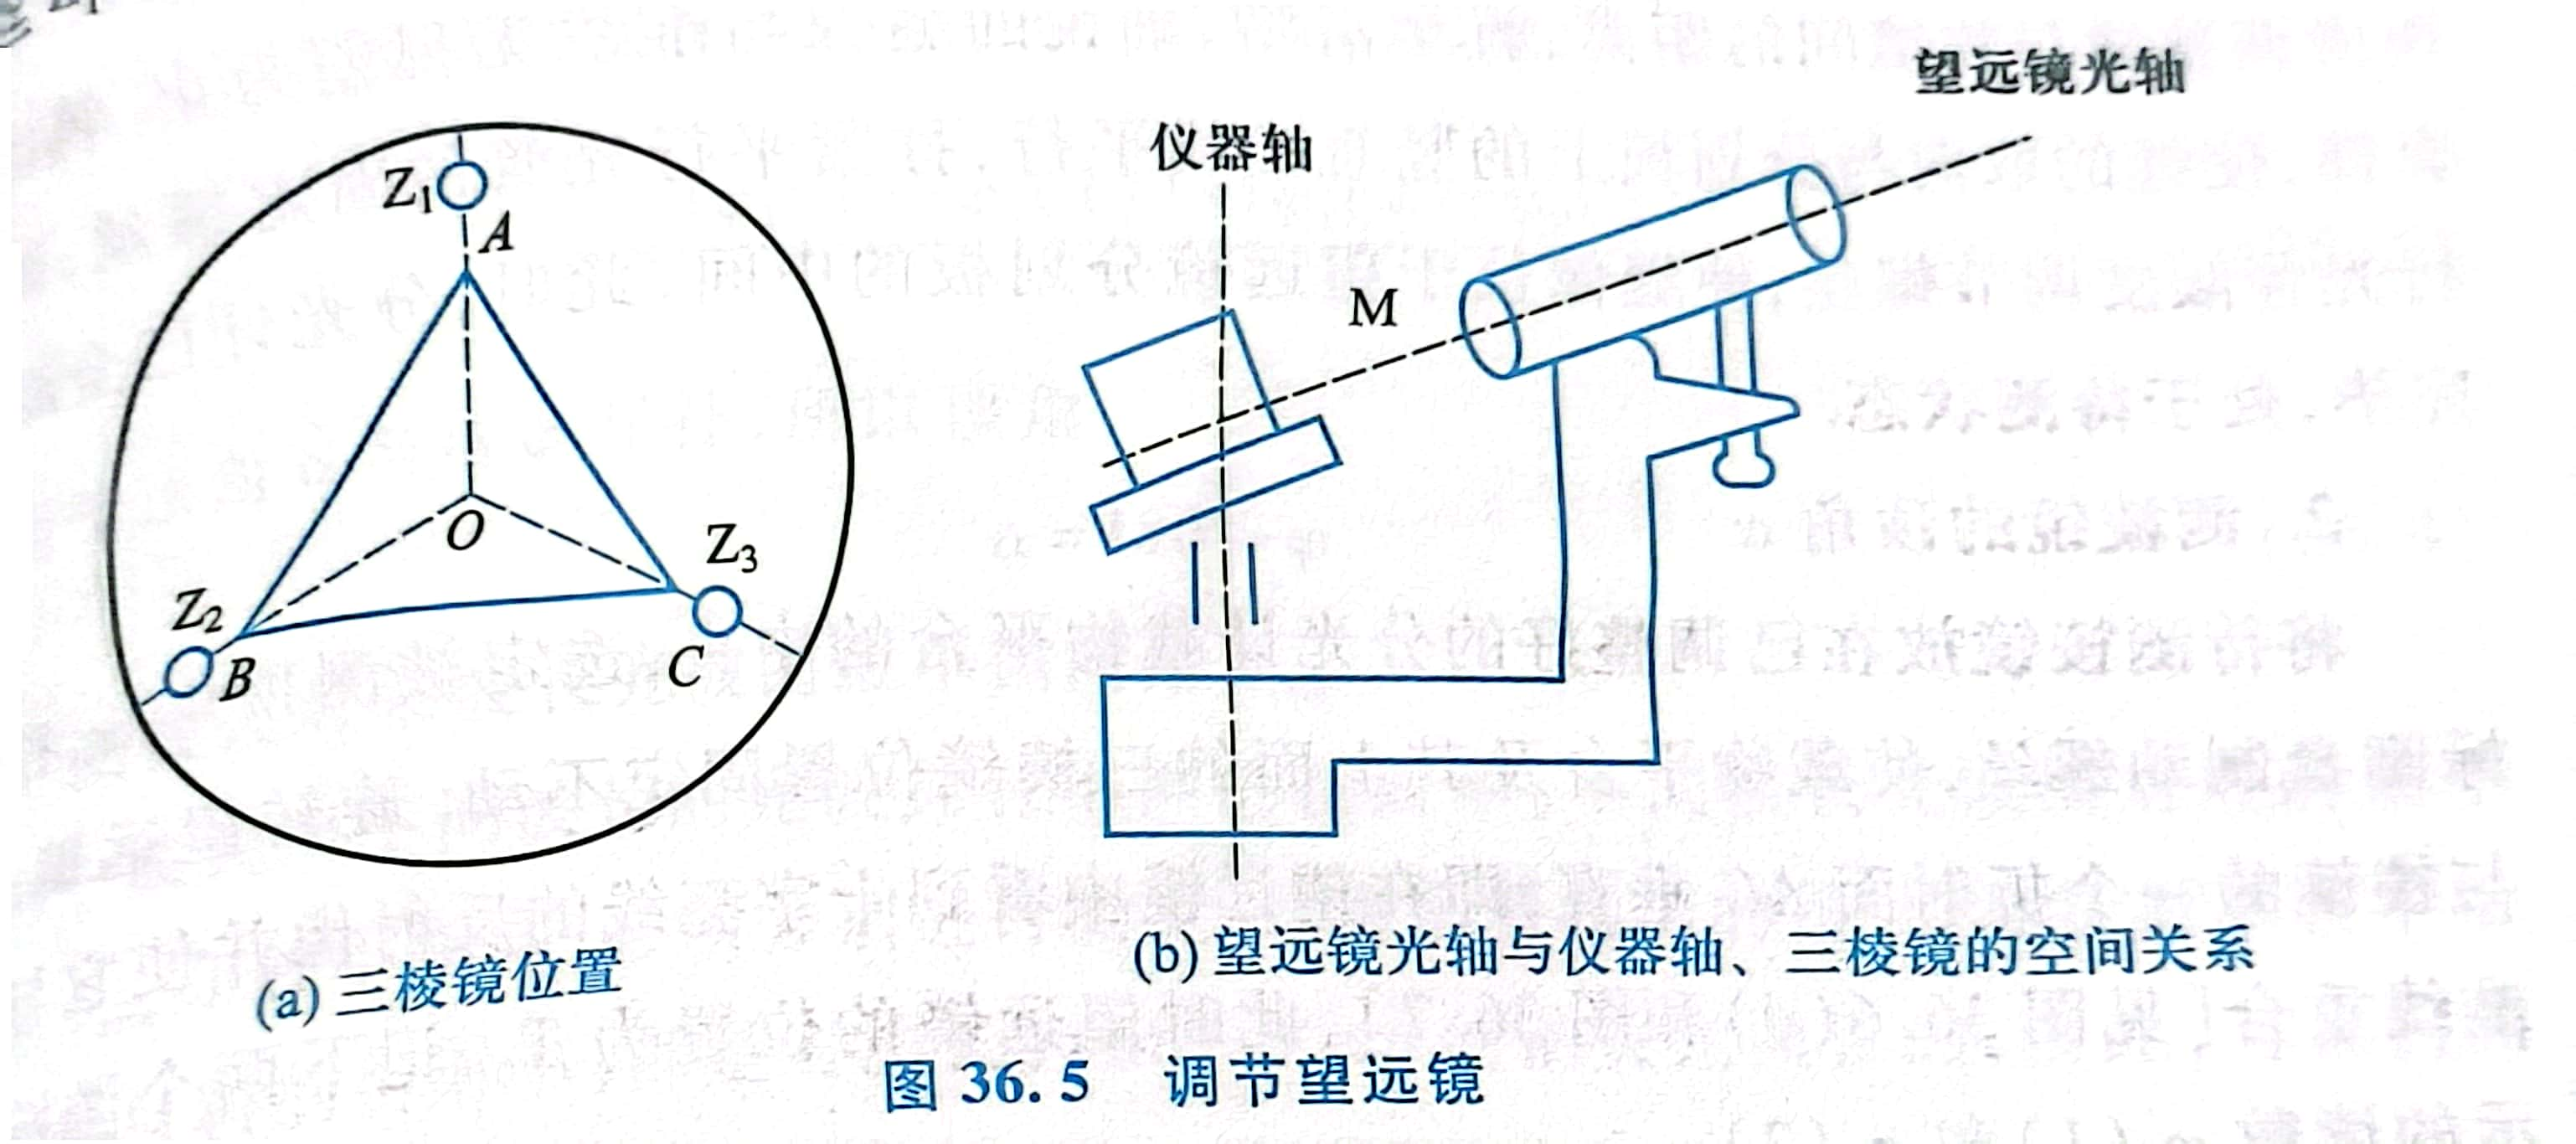
\includegraphics[height=0.5\textwidth,width=1\textwidth]{tiaojiewangyuanjing.jpg}
      \caption{调节望远镜示意图}\label{tiaojiewangyuanjing}
    \end{figure}

    1、 粗调:用目测的方法分别调整望远镜下面的水平调节螺丝和载物平台下面的三个调节螺丝,使望远镜轴和载物平台平面大致处于水平位置。
    2、 细调:将三棱镜按图\ref{tiaojiewangyuanjing}所示放在载物平台上,使三楼镜位于载物平台的中央,
    其水平截面的三个顶点A、B、C分别大致处于平台中心O与平台下三个调节螺丝$Z_{1}$、$Z_{2}$、$Z_{2}$的连线上。

    接下来操作图像可以参考图\ref{wangyuanjingshitu}。

    旋转载物平台,使望远镜对准三棱镜的一个光学面,验证在望远镜中是否能看到亮十字反射像,如果看不到则需要重新进行粗调。
    看到所示的视场后,稍稍转动望远镜使其视场如图所示。调节载物平台下与该面相对的一个调节螺丝,
    使十字反射像的水平位置向分划板上方的水平准线靠拢一半距离,再调节望远镜的俯仰调节螺丝,使亮十字像与分划板上方的十字线重合,
    此时,望远镜轴与该反射面垂直,但不一定和仪器的主轴垂直。因此,必须继续调节。通过旋转游标盘将载物平台转动120°,使望远镜对准棱镜的另一个反射面,
    观察此时亮十字反射像是否仍与分划板上部重合,若不重合,则仍要如上面那样采用二分之一调节法。
    从两方面逼近调节,直到棱镜任一反射面对准望远镜时,亮十字反射像的水平线仍与分划板上部的水平准线重合为止。此时,望远镜光轴已与仪器旋转主轴垂直。
    在仪器调节中,上述二分之一调节法应用很广。
    \begin{figure}[t]
      \centering
      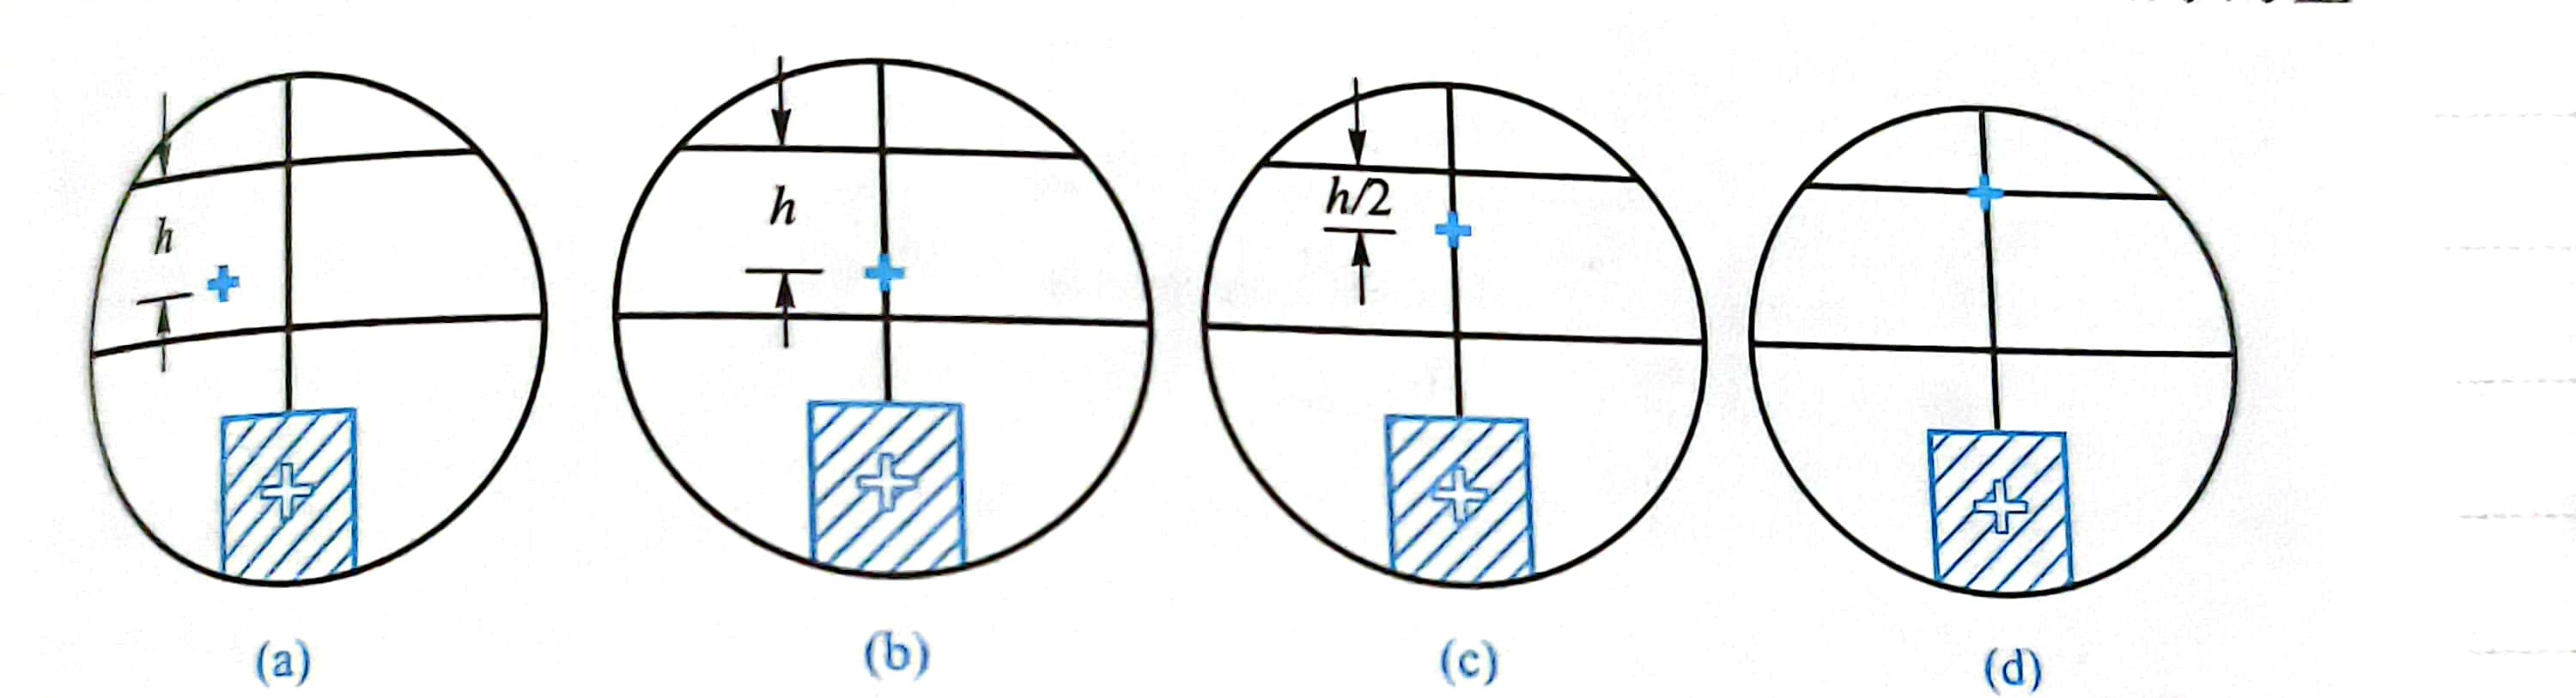
\includegraphics[height=0.4\textwidth,width=1\textwidth]{wangyuanjingshitu.jpg}
      \caption{望远镜视图}\label{wangyuanjingshitu}
    \end{figure}

    \subsubsection{平行光管的调节}
    开启光源,调节照明平行光管的狭缝,取下载物台上的三棱镜,转动调好的望远镜,使它正对着平行光管以观察狭缝的像。
    调节平行光管狭缝与物镜间的距离,在观察到狭缝的清晰像之后,缓慢转动狭缝宽度调节螺丝。
    使缝像既细锐又明亮,再微调狭缝与物镜间的距离,直至清晰、细锐的缝像与准线无视差为止,转动狭缝套简。
    使缝的取向与分划板上的竖直准线平行,拧紧平行光管的固定螺丝,调节平行光管倾度调节螺丝,使缝像位于望远镜分划板的中间。此时,分光计已全部调节完毕,处于待测状态。

    \subsection{测棱镜的顶角$\alpha$}
    示意图可以参考图\ref{cedingjiao}。
    \begin{figure}[H]
      \centering
      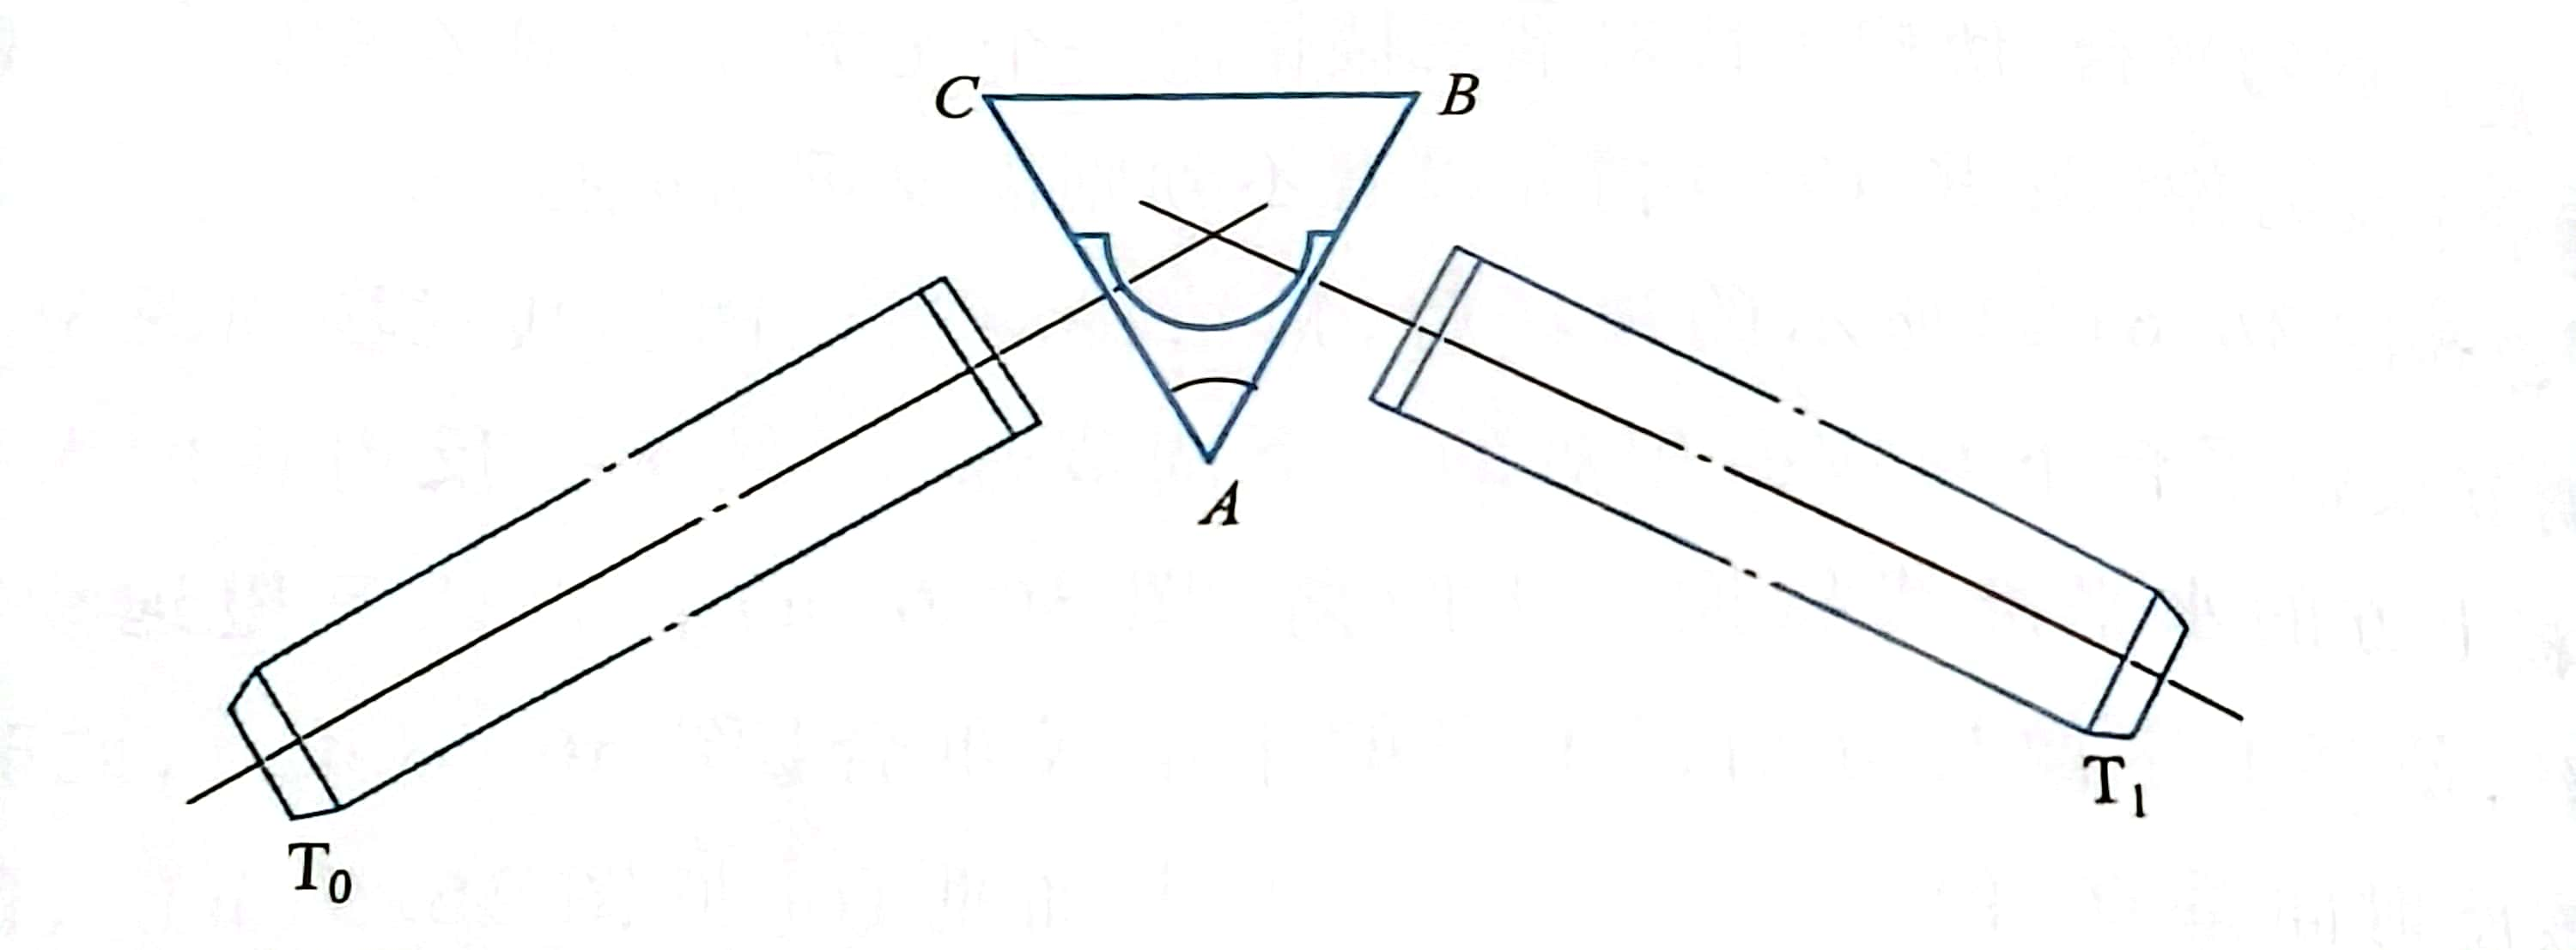
\includegraphics[height=0.2\textwidth,width=1\textwidth]{cedingjiaoguanglu.jpg}
      \caption{测量顶角大小光路示意图}\label{cedingjiao}
    \end{figure}

    将待测棱镜放在已调整好的分光计载物平台的中央,
    选定被测顶角$\alpha$,拧紧游标圆盘制动螺丝,使载物平台及其上面的三棱镜位置固定不动,旋转望远镜,使它与棱镜的一个折射面AC垂直,
    即在望远镜中看到十字亮线的反射像并使它与十字准线重合,此时望远镜的位置为$T_{0}$,记下两个游标所指示的读数$\varphi_{0}(1)$和
    $\varphi_{0}(2)$。

    分光计的读数系统由刻度盘(分度值为0.5°,共360°)和游标盘(分度值为1',共30')组成。读数方法按游标原理进行,
    在图\ref{kedupan}所示的情况下,读数应为87°45'。由于机械加工的原因,刻度盘的中心轴与仪器的旋转主轴不一定重合,
    所以在读数时会出现偏心差,为了消除这种系统误差,读数时应由两个对称安置的游标A和B分别读出后再取平均值.
    \begin{figure}[H]
      \centering
      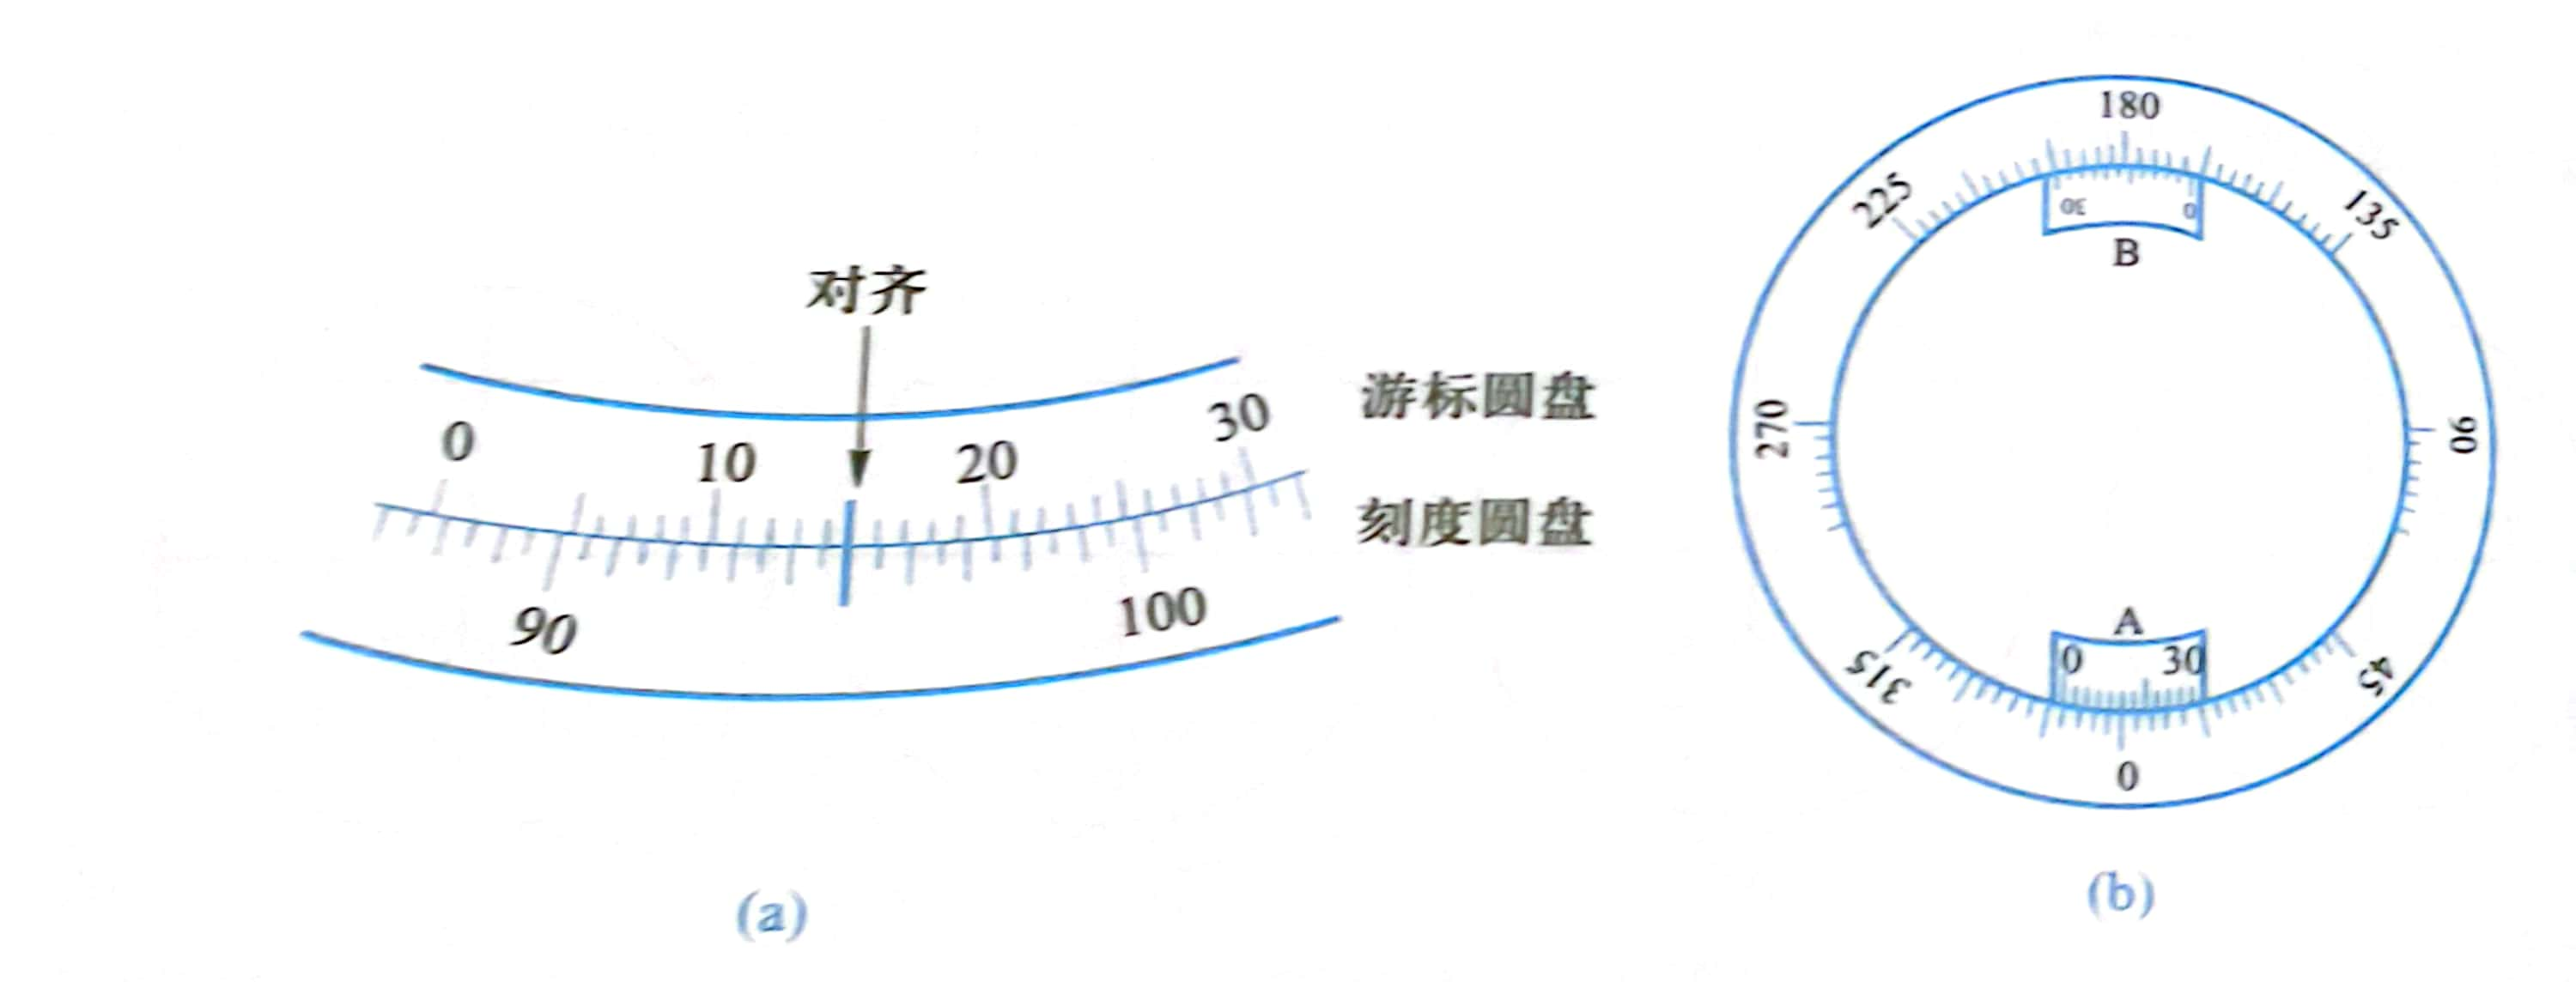
\includegraphics[height=0.4\textwidth,width=1\textwidth]{kedupan.jpg}
      \caption{分光计读数系统}\label{kedupan}
    \end{figure}

    转动望远饶,使它的光轴与梭镜的另一折射面AB垂直,在此位置T上,经AB面反射回来的亮十字像亦与望远镜的十字准线重合,
    记下此时两游标所示的读数$\varphi_{1}(1)$、$\varphi_{1}(2)$。望远镜由位置$T_{0}$转到$T_{1}$,所转过的角度为
    \begin{equation}
      \varphi=\frac{|\varphi_{1}(1)-\varphi_{0}(1)|+|\varphi_{1}(2)-\varphi_{0}(2)|}{2}
    \end{equation}

    由于顶角$\alpha$和角$\varphi$互补,所以顶角等于
    \begin{equation}
      \alpha=180^{\circ}-\varphi
    \end{equation}

    \subsection{测棱镜对某波长光波的最小偏向角$\delta_{min}$}
    同一棱镜对不同波长的光波具有不同的折射率,不同波长光波所对应的最小偏向角$\delta_{min}$亦各不相同。
    必须分别进行测量。这里需要指出的是:以往折射率表中给出的某种材料的折射率。
    都是对波长为589.3 nm的钠黄光而言的。因此,与我们测得的结果并不相同。
    示意图可以参考图\ref{pianxiangjiao}。
    \begin{figure}[H]
      \centering
      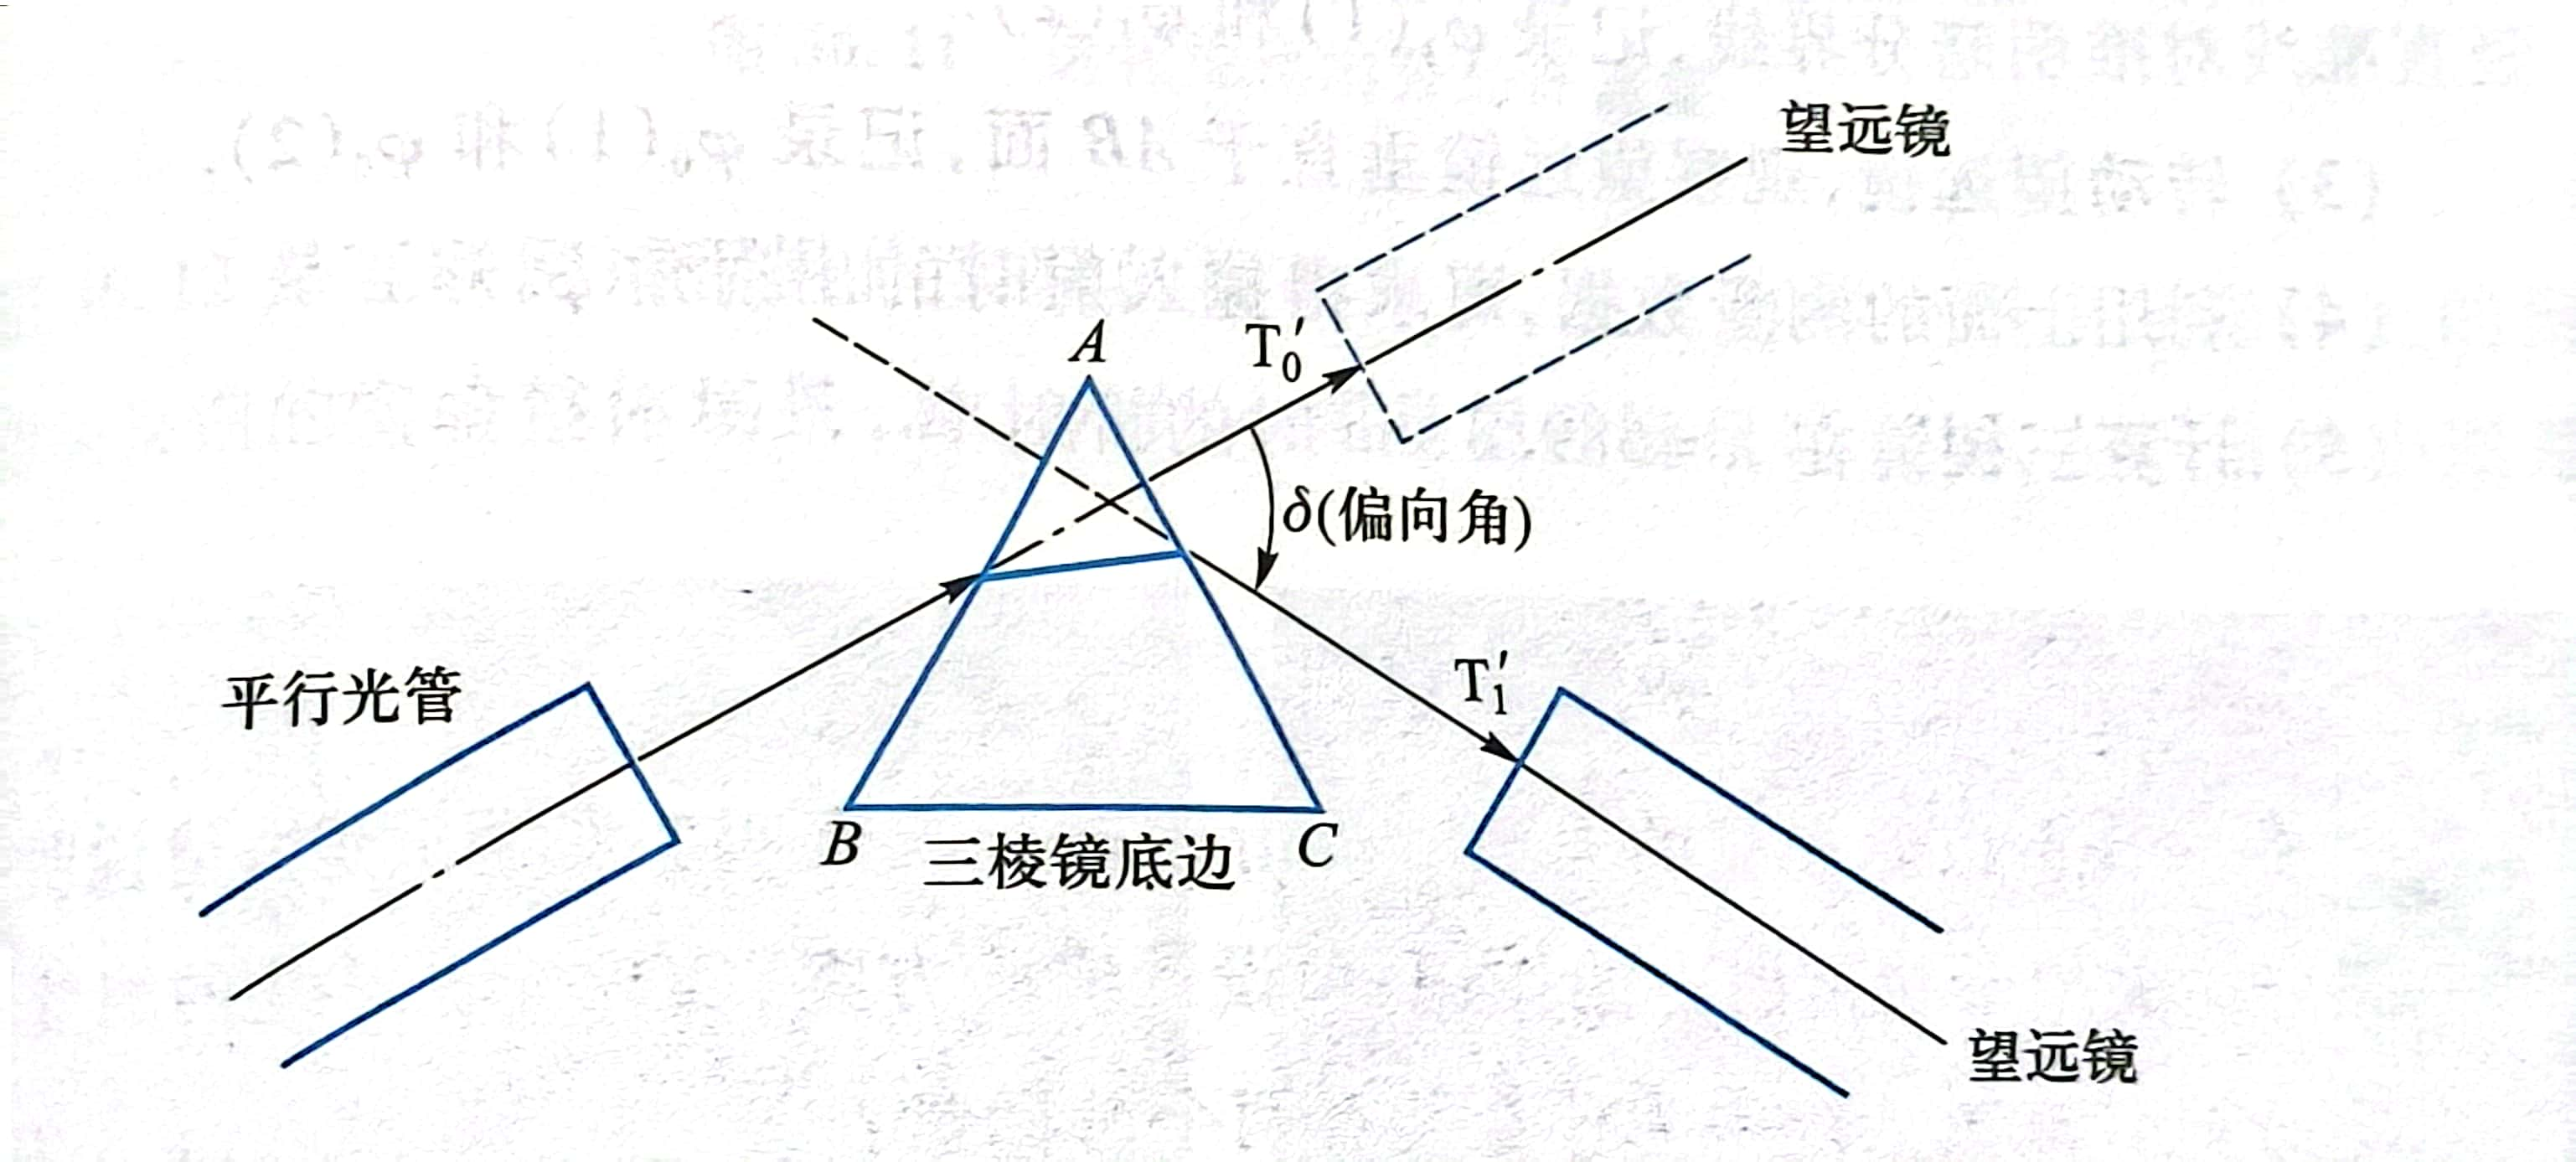
\includegraphics[height=0.3\textwidth,width=1\textwidth]{pianxiangjiaoshiyi.jpg}
      \caption{三棱镜偏向角示意图}\label{pianxiangjiao}
    \end{figure}
    (1)将待测棱镜如图\ref{pianxiangjiao}所示的那样放在载物平台上,开启汞灯光源,
    照明分光计平行光管的狭缝,使平行光管射出的平行光投射到棱镜的折射面AB上.
    使载物平台带动棱镜作适当转动,改变平行光对AB面的入射角,以便观察者可以在$T_{1}^{'}$
    处通过折射面AC直接观察到平行光管管口经棱镜折射所成的虚像I,则各条谱线均在此虚像范围内.

    (2)将望远镜移到T附近,通过它观察汞灯的光谱。
    在看到所有待测谱线后,认定一条谱线,慢慢转动棱镜(即转动载物平台)。
    使该条谱线向$T_{0}^{'}$方向移动(即使谱线向偏向角减小的方向移动)。
    当棱镜转到某一位置时,谱线几乎不再移动,若再使校锁继续沿原方向转动,
    则该谱线反而向相反的方向(即偏向角增大的方向)移动,这个
    转折位置就是梭镜对这条谱线最小偏向角的位置。在找到转折位置后,停止转动棱镜,锁紧载物平台。
    这时平行光的入射角保持不变,所测谱线便固定在最小偏向角的位置$T_{1}^{'}$上。

    (3)缓慢转动望远镜,使它的竖直准线严格对准所认定谱线的中心线,记下两游标的读数$\varphi_{1}^{'}(1)$和$\varphi_{1}^{'}(2)$

    (4)移动望远镜,使其对准狭缝的像(非色散像),当竖直准线位于狭缝像的中心线上时,
    望远镜的光轴便处于人射平行光行进的方向$T_{0}^{'}$上,记下两游标的读数$\varphi_{0}^{'}(1)$和
    $\varphi_{0}^{'}(2)$,望远镜由$T_{1}^{'}$转到$T_{0}^{'}$时所转过的角度就等于棱镜对认定谱线的最小偏向角,即
    \begin{equation}
      \delta_{min}=\frac{|\varphi_{1}^{'}(1)-\varphi_{0}^{'}(1)|+|\varphi_{1}^{'}(2)-\varphi_{0}^{'}(2)|}{2}
    \end{equation}

    (5)用同样的方法测出其他谱线的最小偏向角.

    (6)由式\ref{zheshelv1}算出各波长对所给棱镜的折射率.
\newpage

\section{实验原始数据}
\begin{figure}[H]
  \centering
  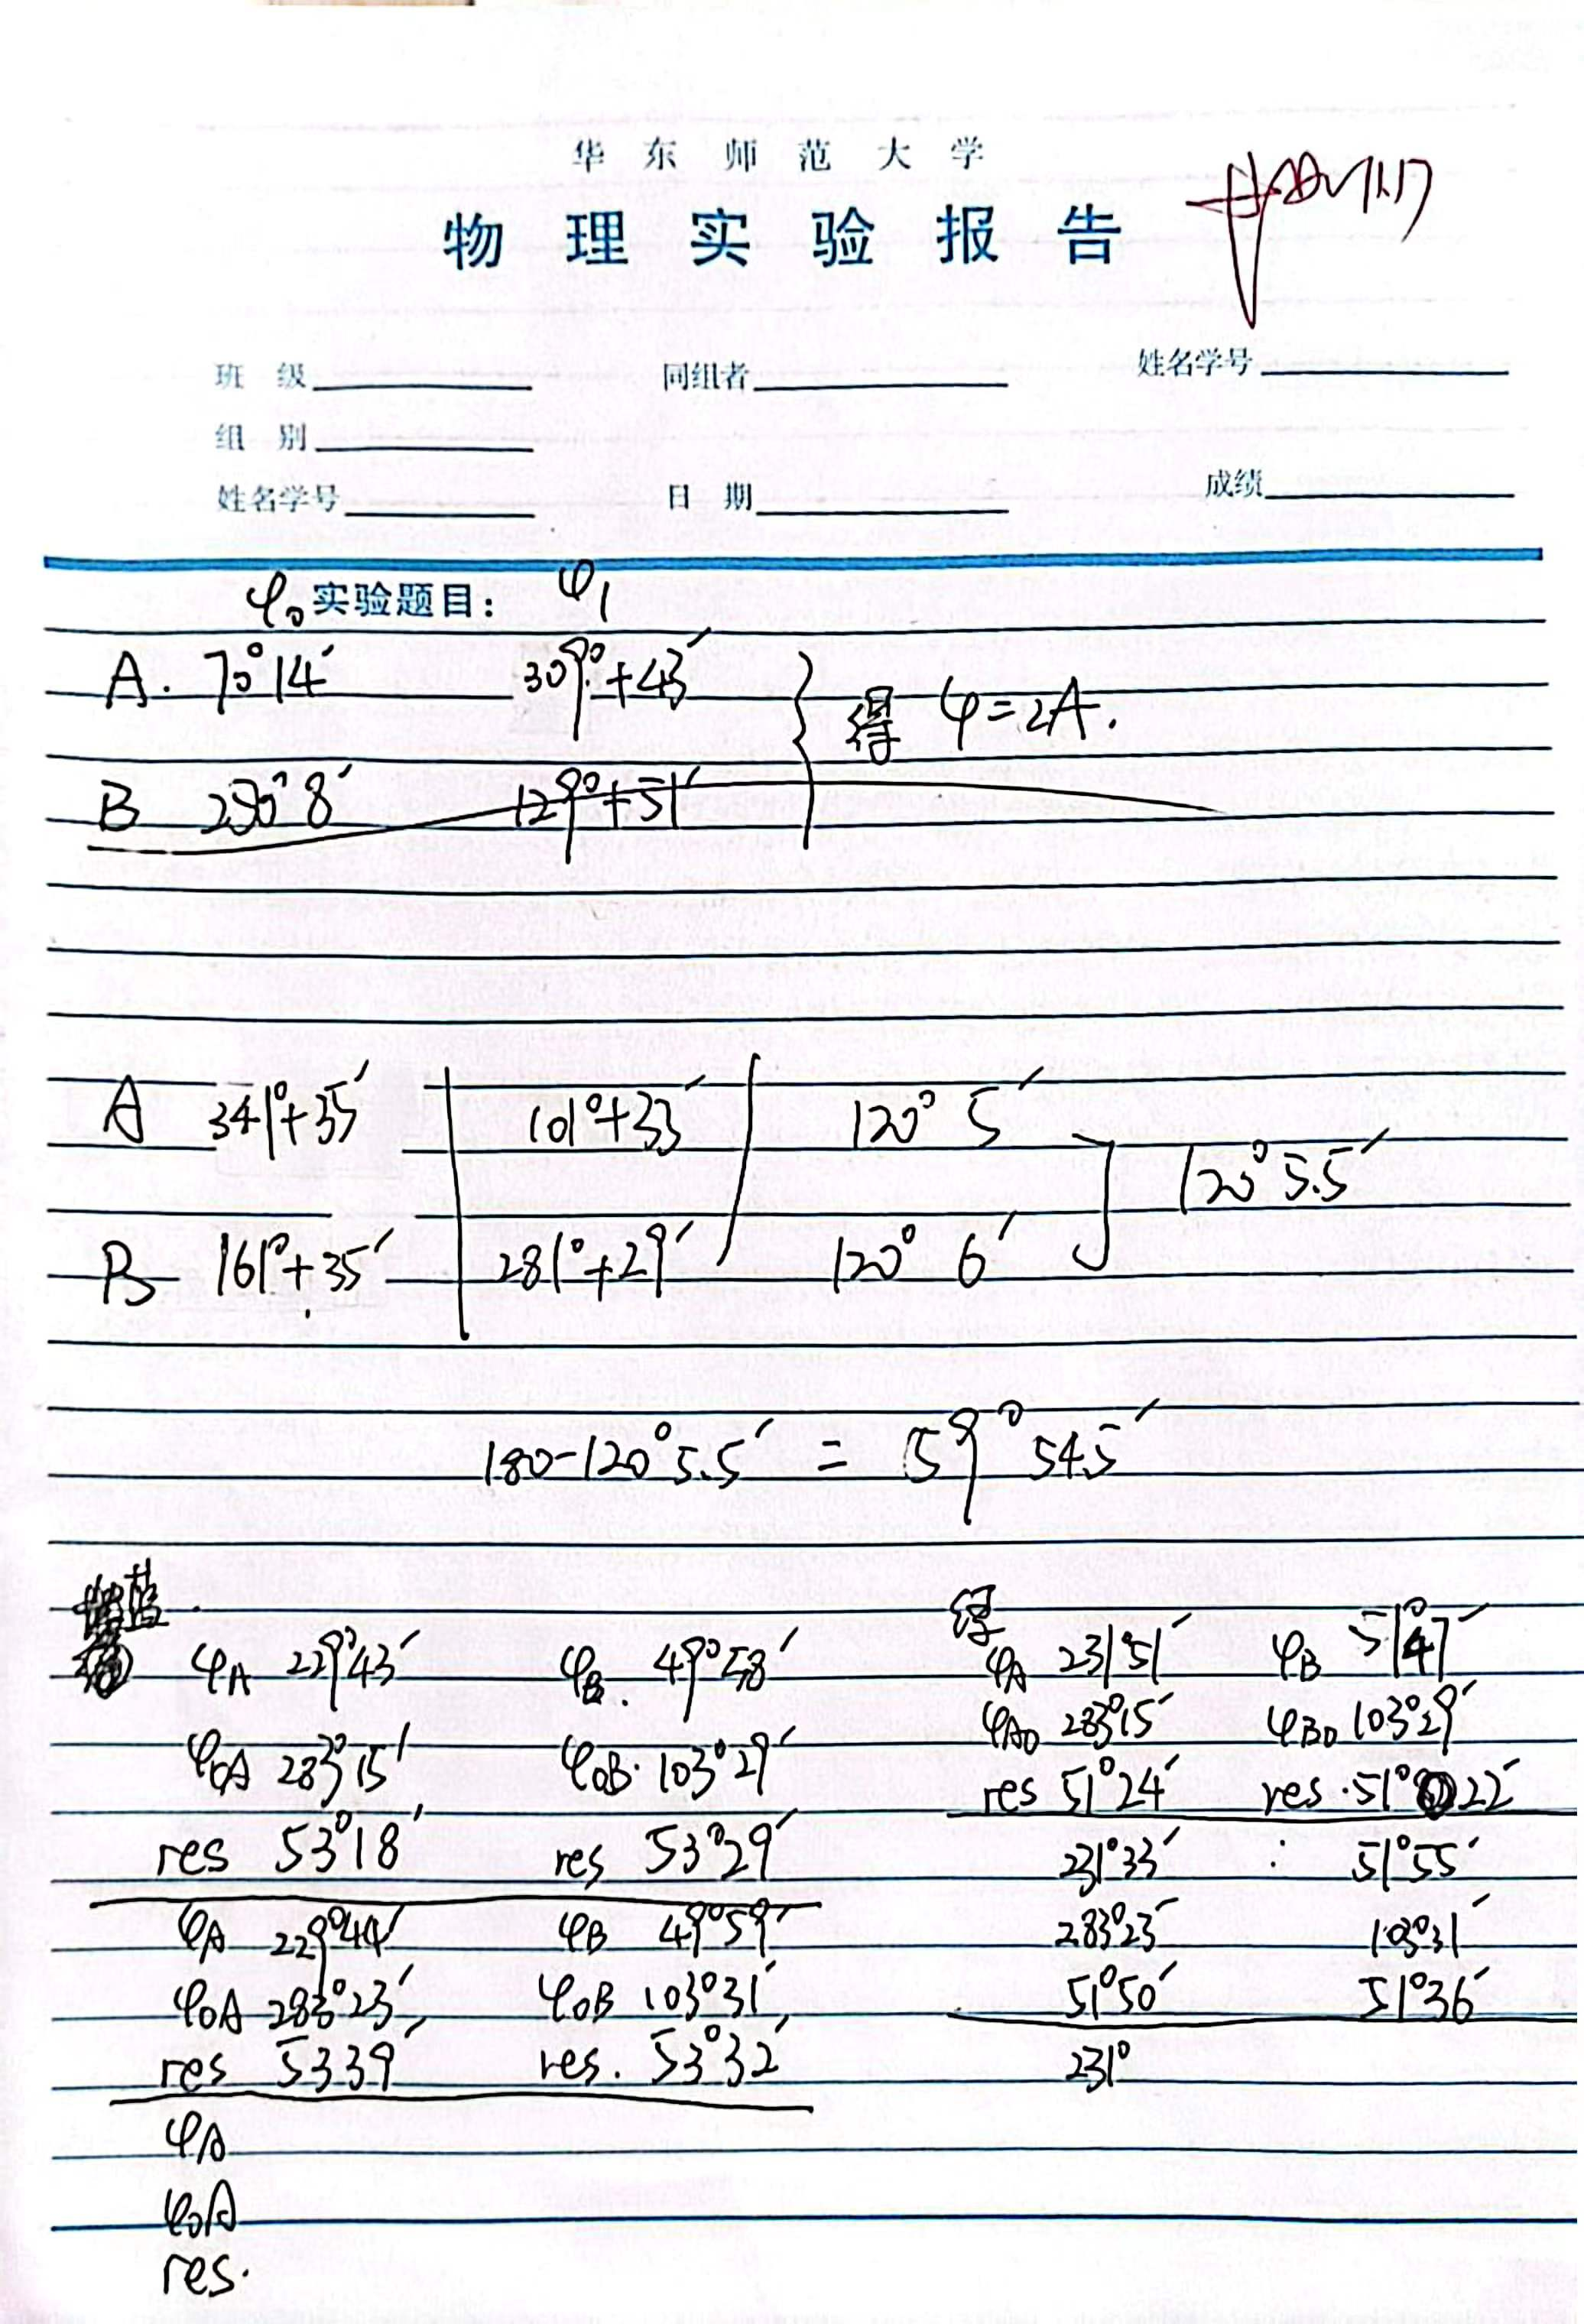
\includegraphics[height=0.8\textheight,width=1\textwidth]{yuanshishujv.jpg}
  \caption{实验原始数据}\label{yuanshishujv}
\end{figure}
\newpage

\section{实验数据处理}
  \subsection{测量顶角大小}
  实验测得数据如表\ref{dingjiaoshujv}所示。
  \begin{table}[H]
    \centering   
    \caption{顶角大小测定与计算}\label{dingjiaoshujv}
    \begin{tabular}{||c|c|c|c|c||}
      \hline
      \hline
      $\varphi_{0}(1)$ & $\varphi_{0}(2)$ & $\Delta\varphi_{0}$ & $\Delta\varphi_{ave}$ & $\alpha$\\
      \hline
      $341^{\circ}35^{'}$ & $101^{\circ}33^{'}$ & $120^{\circ}5^{'}$ & \multirow{3}{*}{$120^{\circ}5.5^{'}$} & \multirow{3}{*}{$59^{\circ}5.5^{'}$}\\
      \cline{1-3}
      $\varphi_{0}^{'}(1)$ & $\varphi_{1}^{'}(2)$ & $\Delta\varphi_{0}^{'}$ & & \\
      \cline{1-3}
      $161^{\circ}35^{'}$ & $281^{\circ}29^{'}$ & $120^{\circ}6^{'}$ & & \\
      \hline
      \hline
    \end{tabular}
  \end{table}
  通过计算可以得到顶角的数值为$59^{\circ}54.5^{'}$。

  \subsection{蓝光光波最小偏向角}
  实验得到的数据及数据处理结果如图\ref{lanpianjiao}所示。
  \begin{figure}[H]
    \centering
    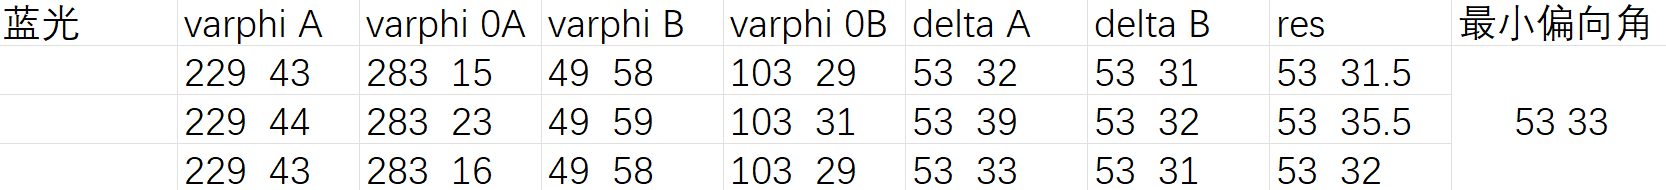
\includegraphics[height=0.1\textwidth,width=1\textwidth]{lanpianjiao.png}
    \caption{蓝光光波最小偏向角数据图}\label{lanpianjiao}
  \end{figure}
  通过结果可以看出最终得到的实验结果为蓝光光波的最小偏向角为$53^{\circ}33^{'}$。

  通过公式计算得到的折射率为
  \begin{equation}
    n=\frac{\sin\frac{59^{\circ}54.5^{'}+53^{\circ}33^{'}}{2}}{\sin\frac{59^{\circ}54.5^{'}}{2}}=1.674
  \end{equation}

  \subsection{绿光光波最小偏向角}
  实验得到的数据及数据处理结果如图\ref{lvpianjiao}所示。
  \begin{figure}[H]
    \centering
    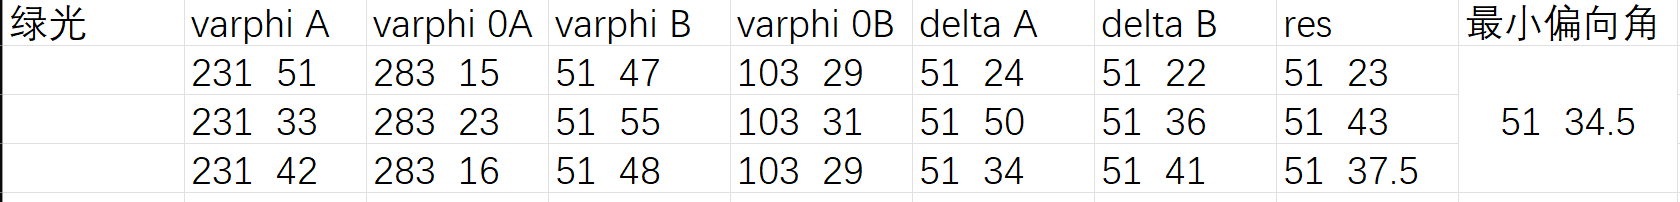
\includegraphics[height=0.1\textwidth,width=1\textwidth]{lvpianjiao.png}
    \caption{绿光光波最小偏向角数据图}\label{lvpianjiao}
  \end{figure}
  通过结果可以看出最终得到的实验结果为绿光光波的最小偏向角为$51^{\circ}34.5^{'}$。

  通过公式计算得到的折射率为
  \begin{equation}
    n=\frac{\sin\frac{59^{\circ}54.5^{'}+51^{\circ}34.5^{'}}{2}}{\sin\frac{59^{\circ}54.5^{'}}{2}}=1.655
  \end{equation}

  \subsection{误差分析}
  \subsubsection{蓝光光波最小偏向角}
  计算可得为$2^{'}45^{"}$。最终结果为$\delta_{min}=53^{\circ}33^{'}\pm 2^{'}45^{"}$。
  \subsubsection{绿光光波最小偏向角}
  计算可得为$4^{'}24^{"}$。最终结果为$\delta_{min}=51^{\circ}34^{'}\pm 4^{'}24^{"}$。

\section{思考题}
  \subsection{夫琅和费衍射中分光计使用}
  可以通过分光计观察到夫琅和费衍射现象。夫琅和费衍射的条件包括光波通过一个有限大小的开口,
  并且开口的尺寸与波长的比值决定了衍射的效果。如果分光计的光源通过一个狭缝或小孔,
  而这个狭缝或小孔的尺寸和光的波长相当,那么就有可能观察到夫琅和费衍射现象。

  具体的实验可以如下设计:

  将光线通过光栅,引发光的衍射。之后调节分光计,直到观察到清晰的衍射级数,再使用分光计进行
  角度的测量。然后再通过夫琅和费衍射关系计算光栅常数。

  \subsection{分光计两个读数盘}
  分光计使用两个读数盘的原因是由于分光计的读数盘和中心轴之间可能存在偏心差,使用两个读数盘进行读数然后
  取平均值的目的就是为了减少偏心差带来的影响。

  \subsection{是否重新寻找最小偏向角位置}
  如果实验器材未发生改变移动,实验仪器也没有改变,在同一条件下测量不同谱线的最小偏向角的时候
  不需要重新寻找最小偏向角的位置。因为最小偏向角的位置和观测无关,在条件不变的情况下是不变的。

  \subsection{棱镜色散光谱和光栅色散光谱特点分析}
  两者相同点有:

  1、都是色散现象,是复合光通过某种特定光学仪器后由于不同光的性质不同导致发生色散的情况。

  2、都会显示出不同颜色的光谱。

  而棱镜色散的图像更加分散,是由于不同光的折射率不同而产生的,所以光谱更加分散,不连续。
  光栅色散是由于衍射现象而产生的色散,更加连续,光谱是连着的。
\newpage

\section{实验中个人的思考与感想}
  \subsection{对于实验个人观点}
  实验中能够测量不同颜色光由于折射产生的偏向角。但是实际中如果分光镜的缝隙太小,则难以观察到现象。
  而分光镜的缝隙太大则在测量中会引入误差,难以找到某一颜色光谱的中心。

  而实验中的预备的调节步骤是极其重要的。如果调节不够准确,则之后连现象都不一定能够观察到。实验非常需要
  耐心进行寻找。调平的二分之一调节法能够较为有效调节调平。

  整个实验并不复杂,需要测量的内容也十分简单,主要是实验器材不方便使用。如果调节不当可能会观察到棱镜色散。
  观察到连续渐变的色散光谱,而调节得当就能观察到实验的结果。非常有趣。

  \subsection{实验中的总结}
  通过实验学习了分光计的使用与调节。并且通过实验观察并测量了不同光的折射率不同的现象和数据。
\end{document}